% Mayuresh Vrushabhanath Pachore Thesis 2025-2026

% ===============================
% Document Class
% ===============================
\documentclass[12pt,a4paper,twoside]{book}

% ===============================
% Encoding & Language
% ===============================
\usepackage[T1]{fontenc}
\usepackage[utf8]{inputenc}
\usepackage[english]{babel}

% ===============================
% Page Layout
% ===============================
\usepackage{geometry}
\geometry{
    left=25mm,
    right=25mm,
    top=25mm,
    bottom=25mm
}

\usepackage{setspace}
\onehalfspacing % or \doublespacing if required

\usepackage{indentfirst}
\usepackage{pdflscape}

% ===============================
% Fonts
% ===============================
\usepackage{lmodern}        % Improved Computer Modern
\usepackage{microtype}      % Better typography

% ===============================
% Mathematics
% ===============================
\usepackage{amsmath}
\usepackage{amssymb}
\usepackage{amsfonts}
\usepackage{amsthm}
\usepackage{bm}             % Bold math symbols
\usepackage{mathtools}

% ===============================
% Graphics & Figures
% ===============================
\usepackage{graphicx}
\usepackage{float}
\usepackage{subcaption}
\usepackage{caption}
\usepackage{tikz}
\usetikzlibrary{arrows.meta,positioning,calc}

% ===============================
% Tables
% ===============================
\usepackage{booktabs}
\usepackage{multirow}
\usepackage{array}
\usepackage{longtable}
\usepackage{tabularx}
\usepackage{rotating}  % Per tabelle orizzontali (sidewaystable)
\usepackage{float}     % Per lo specificatore posizionale [H]

% ===============================
% Algorithms & Code
% ===============================
\usepackage{algorithm}
\usepackage{algpseudocode}

\usepackage{listings}
\usepackage{xcolor}

\lstdefinelanguage{TypeScript}{
  keywords={abstract, any, as, async, await, boolean, break, case, catch, class, console,
    const, constructor, continue, debugger, declare, default, delete, do, else, enum,
    export, extends, false, finally, for, from, function, get, if, implements, import, in,
    instanceof, interface, is, keyof, let, module, namespace, new, null, number, object,
    package, private, protected, public, readonly, require, return, set, static, string,
    super, switch, symbol, this, throw, true, try, type, typeof, undefined, var, void,
    while, with, yield},
  morecomment=[l]{//},
  morecomment=[s]{/*}{*/},
  morestring=[b]',
  morestring=[b]",
  morestring=[b]`
}

\lstset{
    basicstyle=\ttfamily\small,
    keywordstyle=\color{blue},
    commentstyle=\color{green!60!black},
    stringstyle=\color{red},
    numbers=left,
    numberstyle=\tiny,
    frame=single,
    breaklines=true
}


% ===============================
% Units & Symbols
% ===============================
\usepackage{siunitx}
\sisetup{
    per-mode=symbol,
    detect-all
}

% ===============================
% Hyperlinks
% ===============================
\usepackage{hyperref}
\hypersetup{
    colorlinks=true,
    linkcolor=blue,
    citecolor=blue,
    urlcolor=blue
}


% ===============================
% Chapter/Section appearance  (PUT THIS HERE)
% ===============================
\usepackage{titlesec}

% Chapters: small "Chapter X", big title, better spacing
\titleformat{\chapter}[display]
  {\normalfont\bfseries}
  {\Large\chaptername\ \thechapter}
  {5ex}
  {\huge}



% ===============================
% Headings & TOC
% ===============================
\usepackage{chngcntr} % for \counterwithin
\usepackage{tocloft}
\usepackage{fancyhdr}
\pagestyle{fancy}
\fancyhf{}

% -----------------------
% Marks (chapter/section)
% -----------------------
\renewcommand{\chaptermark}[1]{\markboth{\thechapter.\ #1}{}}
\renewcommand{\sectionmark}[1]{\markright{\thesection.\ #1}}

% -----------------------
% Header
% -----------------------
% Left: current chapter/section
\fancyhead[L]{\small\nouppercase{\leftmark}}

% Right: page number (2.1, 2.2 ...)
\fancyhead[R]{\small\thepage}

% -----------------------
% Footer
% -----------------------

% Odd pages -> thesis title on left
\fancyfoot[L]{%
\ifodd\value{page}
\footnotesize \textit{\ThesisTitle}
\fi
}

% Even pages -> course/university on right
\fancyfoot[R]{%
\ifodd\value{page}
\else
\footnotesize \CourseUniversity
\fi
}

% -----------------------
% Lines
% -----------------------
\renewcommand{\headrulewidth}{0.4pt}
\renewcommand{\footrulewidth}{0.4pt}

% -----------------------
% First page of chapters
% -----------------------
\fancypagestyle{plain}{
\fancyhf{}
\fancyfoot[C]{\thepage}
\renewcommand{\headrulewidth}{0pt}
\renewcommand{\footrulewidth}{0pt}
}

% -----------------------
% Unnumbered chapters
% -----------------------
\fancypagestyle{chapterstar}{
\fancyhf{}
\fancyfoot[C]{\thepage}

\renewcommand{\headrulewidth}{0pt}
\renewcommand{\footrulewidth}{0pt}
}

\fancypagestyle{chapterplain}{
\fancyhf{}
\fancyfoot[L]{\footnotesize \CourseUniversity}
\fancyfoot[R]{\footnotesize \thepage}
\renewcommand{\headrulewidth}{0pt}
\renewcommand{\footrulewidth}{0.4pt}
}

\fancypagestyle{chapternum}{
  \fancyhf{}

  % Header
  \fancyhead[L]{\small\rightmark}
  \fancyhead[R]{\small\thepage}

  % Footer
  \fancyfoot[R]{%
    \ifodd\value{page}
      \footnotesize \textit{\ThesisTitle}
    \fi
  }

  \fancyfoot[L]{%
    \ifodd\value{page}
    \else
      \footnotesize \CourseUniversity
    \fi
  }

  \renewcommand{\headrulewidth}{0.4pt}
  \renewcommand{\footrulewidth}{0.4pt}
}

\usepackage[round]{natbib}


% ===============================
% Appendices
% ===============================
\usepackage{appendix}

% ===============================
% Nomenclature / Acronyms
% ===============================
\usepackage{nomencl}
\makenomenclature

% \usepackage[acronym]{glossaries}
% \makeglossaries

% ===============================
% PDF Inclusion
% ===============================
\usepackage{pdfpages}

% ===============================
% Line Breaking & Widow Control
% ===============================
\usepackage[all]{nowidow}

% ===============================
% Custom Commands (optional)
% ===============================
\newcommand{\R}{\mathbb{R}}
\newcommand{\vect}[1]{\boldsymbol{#1}}

\newcommand{\AuthorName}{\textit{Cesidio Rosica}}
\newcommand{\ThesisTitle}{Deep Reinforcement Learning e volatility targeting}
\newcommand{\CourseUniversity}{Laurea Triennale in Informatica, DISI, Universit\`a di Bologna}

\setlength{\headheight}{14pt}

% ===============================
% End of Preamble
% ===============================


\begin{document}

    %Only for title page 
    \setlength{\parindent}{15pt}
    \setlength{\parskip}{15mm}
    
    \begin{titlepage}
        \begin{center}
            
\includegraphics[width=6.5cm,height=4.7cm]{figs/Unibo_Logo.png}
        
            {\large{\bf{Dipartimento di Informatica - Scienza e Ingegneria - DISI }}}
        
            {\Large{\bf{Tesi di Laurea Triennale}}}
        
            {\bfseries\fontsize{20pt}{20pt}\selectfont
                \setlength{\lineskip}{2pt}%
                \setlength{\lineskiplimit}{0pt}%
                Deep Reinforcement Learning e volatility targeting nella gestione dinamica dell'esposizione: un'analisi dei limiti dell'apprendimento\par}
            
        \end{center}
        
        \begin{minipage}[t]{0.5\textwidth}
            {\Large{\bf Relatore: \\ Prof. Federico Montori}}
            \vspace{6mm}

            
        \end{minipage}
        \hfill
        \begin{minipage}[t]{0.40\textwidth}\raggedleft
            {\Large{\bf Candidato: \\ Cesidio Rosica}}
        \end{minipage}

        \rule[0.5mm]{15.3845cm}{0.4mm}
        \vspace{-\baselineskip}
        \begin{center}
            {\large\bfseries Mese Sessione di Laurea Ottobre\\}
            {\large\bfseries Anno Accademico 2025/2026}
        \end{center}

    \end{titlepage}
    \clearpage{\pagestyle{empty}\cleardoublepage}

    \pagenumbering{roman} %page numbering is roman letters for this section
    \setlength{\parindent}{15pt}
    \setlength{\parskip}{0pt}
    

        
	\chapter*{Riassunto}
    \addcontentsline{toc}{chapter}{Riassunto}
    \thispagestyle{chapterstar}
	\label{abstract_It}
	% !TEX root = main.tex
Questo lavoro indaga se la componente appresa di un agente di Deep Reinforcement Learning aggiunga valore rispetto a una regola strutturale fissa che punta a regolare l'esposizione al mercato. 
L'agente addestrato con PPO su una rete ricorrente (GRU) e con politica basata su una distribuzione Beta, non sostituisce la strategia di volatility targeting di Moreira e Muir ma la corregge attraverso un unico moltiplicatore appreso $m_\theta$.
La selezione dei titoli è congelata a equal-weight in modo da isolare la sola decisione di esposizione e permettere un confronto pulito tra ciò che la rete impara e ciò che la formula fornisce.

Il modello è valutato out-of-sample su più regimi di mercato e su panieri diversi, con protocollo multi-seed e una frontiera di controllo a parità di liquidità media. 
I risultati mostrano che la parte appresa non aggiunge nulla che non si possa ottenere scegliendo i parametri strutturali fissi. 
Il minor drawdown dell'agente deriva dal mantenere più liquidità, non da un reale tempismo, l'agente quindi non ha svilupato alcun tipo d'intelligenza di market timing. 
L'agente ricade sulla frontiera della regola deterministica, resta dominato sullo Sharpe e la dipendenza dal regime dell'esponente non è sfruttabile in tempo reale.
La ragione è economica: la volatilità è prevedibile, la direzione del mercato no.

Il contributo non è dimostrare che l'apprendimento batte una regola, ma quantificare con rigore, tramite ablation e controlli, il limite dell'adattività appresa in un dominio a basso rapporto segnale/rumore. 
Come obiettivo secondario è stata sviluppata un'applicazione mobile local-first che esegue il modello on-device, rendendo le strategie studiate concretamente utilizzabili.

	\clearpage{\pagestyle{empty}\cleardoublepage}
	
	

    \pagestyle{chapterstar}
    \chapter*{Acknowledgment}
    \addcontentsline{toc}{chapter}{Acknowledgment}
    \thispagestyle{chapterstar}
	\label{acknow}
	% !TEX root = main.tex
First and foremost, I would like to express my sincere gratitude to my supervisor, Prof. [Supervisor's Name], for their invaluable guidance, patience, and continuous support throughout the course of this work. Their expertise and insightful feedback have been instrumental in shaping both the direction and quality of this thesis.
I am deeply grateful to the Department of [Department Name] at the Alma Mater Studiorum – Università di Bologna for providing the academic environment and resources that made this research possible.
I would also like to thank my colleagues and fellow students for the stimulating discussions, shared knowledge, and moments of encouragement during the challenging phases of this journey. Their companionship made the experience all the more rewarding.
A special thanks goes to the open-source LaTeX community, whose collective efforts and freely shared tools and packages have greatly facilitated the preparation of this document. This template itself stands as a testament to the spirit of collaborative academic contribution.
Finally, and most profoundly, I wish to thank my family and friends for their unwavering love, moral support, and belief in me — especially during the most demanding moments of this academic pursuit. This work would not have been possible without them.
	\clearpage{\pagestyle{empty}\cleardoublepage}
	
		
	
	%table of contents
    \tableofcontents
    \thispagestyle{chapterstar}
    \clearpage
    \pagestyle{fancy}
    \cleardoublepage

    \addcontentsline{toc}{chapter}{List of Figures}
	\listoffigures
    \thispagestyle{chapterstar}
	\clearpage{\pagestyle{empty}\cleardoublepage}

    \listoftables
    \thispagestyle{chapterstar}
    \addcontentsline{toc}{chapter}{List of Tables}
    \clearpage{\pagestyle{empty}\cleardoublepage}

    

    \mainmatter 
    \pagestyle{chapternum}
    
    \pagenumbering{arabic}
    \counterwithin{page}{chapter}
    \renewcommand{\thepage}{\thechapter.\arabic{page}}
    
	\chapter{Introduzione}
    \thispagestyle{chapterplain}
	\label{chap:introduction}
	% !TEX root = main.tex
%=============================================================
% CHAPTER 1: INTRODUCTION
%=============================================================

Il position sizing, ovvero la decisione di quanto capitale investire in un dato titolo e momento, costituisce 
una variabile importantissima per la preservazione del capitale e la stabilità dei rendimenti nel lungo periodo.
Un guadagno molto grande derivato da un titolo su cui abbiamo investito una quantità piccola del nostro capitale risulterà essere marginale nel valore complessivo del portafoglio.
Mentre allocare gran parte del capitale su un titolo che è molto instabile potrebbe compromettere l'intero portafoglio.
Per questo motivo è molto importante spartire il proprio capitale in maniera sensata nel momento in cui si va a investire.
Nel lavoro di \citet{blotnick2025power} si affrontano alcuni problemi che possono incorrere quando si prova a fare position sizing affidandosi al puro intuito, come:
\begin{itemize}
    \item \textbf{Eccesso di fiducia}: porta a concentrare eccessivamente il capitale sui titoli che si è convinti vadano bene, sottostimando le probabilità di crollo.
    \item \textbf{Avversione alle perdite}: è la tendenza a vendere le proprie posizioni in profitto per incassare il prima possibile il guadagno, lasciando d'altra parte ferme le posizioni in perdita sperando in un recupero aumentandone così il peso complessivo nel portafoglio.
    \item \textbf{Pregiudizio di recency}: è ciò che induce a investire di più in fasi rialziste prolungate e a disinvestire drasticamente nei ribassi successivi.
\end{itemize}

Per evitare questi problemi, la ricerca finanziaria ha sviluppato metodologie di dimensionamento della posizione.
I primi approcci sono stati quelli a capitale fisso come l'Equal Weight in cui si divide semplicemente il capitale equamente fra i titoli scelti.
Questi metodi sono molto semplici e addirittura profittevoli ma non offrono alcuna protezione dai rischi di crollo del mercato.
Il mercato azionario infatti è contrassegnato da repentini cambiamenti di stato e dalla tendenza della volatilità a persistere nel tempo.
Osservando questa struttura è diventato necessario sviluppare metodologie di posizionamento dinamiche guidate dal rischio.
Questo lavoro si è basato sulla formula del volatility targeting proposta da Moreira e Muir~\cite{moreira2017volatility}. Essa scala l'esposizione al mercato in proporzione inversa alla volatilità stimata
cioè investe nei periodi in cui la volatilità è bassa e ritorna in liquidità nei momenti in cui quest'ultima si alza.

\section{Stato dell'arte}
\label{subsec:stateofart}
Durante gli anni la gestione del portafoglio ha attraversato una profonda evoluzione. 
Si è partiti da modelli analitici statici fino ad arrivare ad architetture adattive basate sull'intelligenza artificiale.
Tradizionalmente l'allocazione del capitale si è fondata su modelli di ottimizzazione media-variana di Markowitz, essi consistevano nel capire quanta percentuale di capitale investire in ongi titolo in base alla media dei rendimenti attesi e alla loro volatilità, cercando l'allocazione ottimale che massimizzi la prima e minimizzi la seconda.
In seguito si è evoluta verso politiche focalizzate sulla gestione del rischio come il Volatility Targeting.
Queste formule hanno riscontrato un grande successo in quanto sono trasparenti è facile capire il perché delle loro azioni, e si sono dimostrate molto efficienti nell'obiettivo di proteggere il capitale.
Tuttavia esse si basano su regole fisse che non riescono ad'adattarsi dinamicamente ai velocissimi cambi di regime del mercato.
Per far fronte a questo problema negli ultimi dieci anni la ricerca si è mossa verso l'applicazione del Deep Reinforcement Learning (DRL).
Questa a differenza dell'apprendimento supervisionato non tenta di prevedere le direzioni future del mercato che si è dimostrato inefficace, 
ma fa si che un'agente agisca direttamente con l'ambiente di mercato apprendendo una politica di allocazione tramite tentativi ed errori per massimizzare un segnale di reward, quest'ultimo tipicamente basato su metriche corrette per il rischio come lo Sharpe o il Calmar.
Attualmente lo standard impiega algoritmi Actor-Critic come il Proximal Policy Optimization (PPO), per gestire lo spazio di azioni continue richiesto
per calibrare i pesi di un portafoglio. I modelli come DeepTrader\citep{wang2021deeptrader} e MARS \citep{chen2026mars} rappresentano la frontiera di questo approccio integrando l'estrazione di feature macroeconomiche e indicatori di rischio direttamente all'interno dello stato osservato dall'agente, questo nel tentativo di rendere l'agente consapevole delle turbolenze presenti in ogni momento nel mercato.
Purtroppo però l'attuale stato dell'arte è dominato da architetture monolitiche end-to-end, ovvero architetture enormi che prendono i dati grezzi e forniscono direttamente in output il vettore di allocazione dei pesi. 
In questo modo però non è possibile identificare con precisione la reale aggiunta dell'aprendimento rendendo impossibile quantificare e giustificare un miglioramento dato da un modello rispetto alle normali formule fisse.


%-------------------------------------------------------------
\section{Definizione del problema}
\label{sec:problem}
%-------------------------------------------------------------

Nonostante al giorno d'oggi vengano pubblicati innumerevoli studi su architetture di Deep Reinforcement Learning per l'allocazione dinamica del portafoglio.
La letteratura della finanza quantitativa soffre di una mancaza di rigore metodologico nella fase di validazione e test.
Molti di questi studi infatti tendono a riportare solo dei singoli scenari di backtest in cui l'agente batte il benchmark fissato.
Questa impostazione però presenta dei punti critici che sono invece stati toccati in questo lavoro:
\begin{itemize}
    \item \textbf{Scelta dei benchmark}: Molto spesso il confronto avviene solo con strategie 
    passive come l'equal-weight o il buy\&hold, e quasi mai a parità di rischio. Per avere dei risultati legittimi il benchmark dovrebbe essere ovviamente coerenrte
    con l'obiettivo del modello ma è importe anche che sia confrontato a parità di rischio. Questo confronto equo permette di capire meglio se le performance dei vari modelli siano
    gonfiate o meno dal fatto che assumano un rischio maggiore nelle loro allocazioni.
    \item \textbf{Varianza e seed multipli}: I risultati sono spesso presentati con un unico backtest vincente senza esplicitare che siano stati fatti test con più seed.
    Quando si vanno a fare molti backtest provando diverse combinazioni di parametri e paniere è possibile che per puro caso si sia incontrata una configurazione vincente, ma che poi essa non lo sia altrettanto testandola fuori campione.
    Senza avere dati da più backtest e seed che ci indicano quanto sia stabile il modello non possiamo dire se sia stato fatta una scelta del migliore o meno.
    \item \textbf{Ablation dello spazio di azione}: L'agente è quasi sempre una rete monolitica end-to-end e manca un test che isoli il contributo della componente appresa, ovvero che la confronti con una regola semplice, non appresa, capace di svolgere la stessa funzione. Senza questo controllo non è possibile stabilire se il vantaggio derivi davvero dall'apprendimento o da un effetto banale.
\end{itemize}

Per dimostrare la veridicità di questa affermazione sono stati presi 5 paper che si avvicinano al modello implementato in questo lavoro.
Questi documenti sono stati analizzati per vedere se le criticità riportate di sopra sono presenti almeno in parte in essi.
Di sotto si riporta una tabella che sintetizza i risultati di questa ricerca:



\begin{table}[H]
\centering
\small
\renewcommand{\arraystretch}{1.4}
\label{tab:sota-critica-affini}
\begin{tabular}{p{4.3cm} p{2.4cm} p{2.3cm} p{2.4cm}}
\toprule
\textbf{Paper / Autori} & \textbf{Benchmark a parità di rischio?} & \textbf{Multi-seed?} & \textbf{Ablation?} \\
\midrule
Zhang, Zohren \& Roberts (2020) & Sì (vol scaling 10\%) & Non spec.\ & Parziale \\
DeepTrader --- Wang et al.\ (2021) & No & Non spec.\ & Sì (interna) \\
Jung \& Oh (2025) & No & No (seed 42) & Sì (interna) \\
Lwele et al.\ (2025) & No & Non spec.\ & No \\
MARS --- Chen, Li \& Wang (2026) & No & No (seed 42) & Sì (interna) \\
\bottomrule
\end{tabular}
\end{table}

Da questa ricerca emergono tre osservazioni principali.
\begin{enumerate}
    \item In nessuno dei cinque lavori è citato un addestramento su più seed
    indipendenti con medie e intervalli di confidenza; l'unico che fa qualcosa di
    simile è \citet{jung2025factor}, con un ricampionamento Moving-Block Bootstrap
    ex-post.
    \item Gli studi di ablation compaiono nei lavori
    \citep{wang2021deeptrader, jung2025factor, chen2026mars}, ma restano interni:
    isolano quale componente, reward o architettura contribuisca, senza però
    confrontare la componente appresa con una regola semplice, non appresa, capace
    di svolgere la stessa funzione.
    \item Solo \citet{zhang2020deeplearning} applica un confronto a parità di
    rischio, normalizzando in modo uniforme la volatilità di tutti i modelli e
    garantendo così la parità del budget di rischio nel confronto.
\end{enumerate}


Alcuni casi sono particolarmente istruttivi. \citet{lwele2025riskaware} mostra come dopo l'addestramento le prestazioni collassano (Sharpe da $1.41$ a $0.13$),
perché l'agente si limita a tagliare la volatilità perdendo rendimento, pura conservatività, per giunta aggravato da un evidente look-ahead bias nella
selezione del paniere. \citet{wang2021deeptrader} e \citet{chen2026mars} sono i più
simili a questo lavoro, hanno una reward orientata al drawdown e un de-risking guidato
dallo stato del mercato. La loro ablation però resta interna non isolando il contributo
dell'apprendimento rispetto a una regola. \citet{jung2025factor} è il più trasparente, ammette che nel mercato delle criptovalute
la sovraperformance non sopravvive alla verifica bootstrap.







\subsection{Obiettivi e limiti}
\label{subsec:scope}

\subsubsection{Obiettivo primario}
Dopo aver essplorato queste mancanze presenti in molti lavori della finanza quantitativa si è definito lo scopo di questo lavoro.
L'obiettivo è esplorare i limiti effettivi dell'intelligenza artificiale nel position sizing, in particolare nel regolare l'esposizione del capitale al mercato.
La domanda di questa ricerca non è se una rete riesce a battere il mercato ma bensì:

\emph{"La componente appresa agigunge valore rispetto a una regola strutturale fissa nella decisione dell'esposizione?"}

Per rispondere in maniera rigorosa adottiamo i controlli che nei lavori esaminato non compaiono, spiegati nel dettaglio nei prossimi capitoli.



\subsubsection{Limiti}
Tutte le conclusioni in questo lavoro valgono all'interno di confini precisi.
L'universo di riferimento è quello dei titoli large-cap dell'indice S\&P500, cioè le 500 aziende americane con il valore economico più grande.
La selezione dei titoli è congelata a equal-weight isolando in questo modo la sola decisione di esposizione.
L'obiettivo è il contenimento del drawdown non massimizzare il rendimento.
La valutazione è confinata ai periodi e ai regimi di mercato considerati.
I risultati vanno quindi letti come un caso illustrativo di un principio generale e non come un verdetto universale sull'intelligenza artificiale in finanza.
Su mercati
strutturalmente meno efficienti (small-cap, mercati emergenti, cripto-attività), o
in problemi dove la selezione cross-asset è determinante, il margine per
l'apprendimento potrebbe riaprirsi.

\subsubsection{Obiettivo secondario}
Oltre all'obiettivo citato di sopra in questo lavoro è resente anche un secondo obiettivo che implementa una componente applicativa.
Quest'obiettivo consiste nella realizzazione di un'applicazione per la gestione del portafoglio che integra il modello studiato, rendendolo utilizzabile in modo concreto.
La sua architettura e implementazione sono descritte nel dettaglio nel capitolo %~\ref{cap:applicazione}




	\clearpage{\pagestyle{empty}\cleardoublepage}
	
    \chapter{Fondamenti Teorici}
    \thispagestyle{chapterplain}
	\label{chap:backgrounds}
	% !TEX root = main.tex


In questa sezionie vengono fornite al lettore tutte le nozioni di base che servono per comprendere il modello e gli esperimenti.

\section{Fondamenti economici}

\subsection{Gestione del portafoglio}

Gestire il portafoglio significa distribuire il capitale tra un insieme di asset e aggiornarne l'allocazione nel tempo. Ad ogni istante $t$ l'allocazione del portafoglio è un vettore di pesi $w_t$ non negativi che sommano a 1. 
Gli asset veri e propri sono affiancati da un asset fittizio cash che corrisponde alla liquidità, cioè tutto quel capitale che si decide di non investire. 
Si definisce esposizione $e_t$ la quota complessiva investita nel paniere di asset veri e propri, mentre la parte restante ($1-e_t$) resta in liquidità. 
Il rendimento del portafoglio in un dato periodo equivale alla media dei rendimenti degli asset pesata per $w_t$. 

Ogni ribilanciamento comporta inoltre costi di transazione in proporzione al volume scambiato. Questi costi includono le commissioni e lo slippage, ovvero la differenza tra il prezzo osservato nel momento in cui si decide di acquistare e il prezzo effettivo a cui avviene la transazione. 
Modellare questi costi è essenziale per un confronto equo, poiché vanno a penalizzare le strategie con un turnover eccessivo. Il turnover è un termine con cui si indica la frequenza e il volume con cui i vari asset vengono comprati e venduti nel portafoglio in un dato periodo, solitamente misurato su base annuale.

\subsection{Volatilità e drawdown}

La volatilità misura l'ampiezza tipica delle oscillazioni di prezzo attorno alla loro media, quantificando il grado di incertezza e turbolenza a cui è esposto il portafoglio.
Cioè prendendo come esempio un titolo che ha un prezzo attuale di 100\$, se esso ha una volatilità annua del 5\% vuol dire che è molto probabile che quel titolo tra un anno avrà un prezzo che oscilla in un range ±5\%.

A differenza della direzione dei prezzi che è quasi impossibile da prevedere giorno per giorno, la volatilità tende a raggrupparsi nel tempo. Giornate con alta turbolenza sono sistematicamente seguite da altre fasi agitate, e i periodi di calma tendono a persistere nel tempo. Tutto questo rende la volatilità prevedibile. 

Questa asimmetria tra la volatilità e la direzione rende economicamente utile agire sul rischio invece che sul rendimento~\cite{fleming2001economic}.

Il drawdown $\mathrm{DD}_t$ è la perdita corrente rispetto al massimo storico del portafoglio. La formula è $(\text{picco}-V_t)/\text{picco}$ e il suo massimo (MDD) è il suo valore peggiore. Esso è la misura di perdita più importante per un investitore ed è l'obiettivo centrale di questo lavoro.

\subsection{Volatility targeting}
Il volatility targeting è una regola classica di gestione del rischio: si scala l'esposizione in modo inversamente proporzionale alla volatilità di mercato, così da tenere il rischio del portafoglio vicino a un livello obiettivo $\sigma_\text{target}$. Nella forma generale l'esposizione e'
$e_t = (\sigma_{\text{target}}/\sigma_{\mathrm{mkt},t})^{p}$: con $p=1$ si
ha il volatility targeting classico ($1/\sigma$), Moreira e Muir applicano invece $p=2$ ($1/\sigma^2$), che riduce l'esposizione in modo piu'
aggressivo quando la volatilita' sale. Sempre Moreira e Muir~\cite{moreira2017volatility}
mostrano che gestire l'esposizione sulla volatilita' realizzata migliora il
profilo rischio/rendimento: e' la regola strutturale che fa da riferimento in
tutto il lavoro. 
\subsection{Dividendi}
Un dividendo è una porzione degli utili aziendali che la socièta decide di non reinvestire internamente, ma di fornire in contanti ai propri azionisti come pagamento.
Il meccanismo funziona in questo modo: nel giorno in cui avviene il dividendo il denaro esce dai bilanci dell'azienda e il prezzo dell'azione in borsa scende di un importo pari al dividendo pagato.
Per esempio se un'azione è quotata in borsa a 100\$ e paga 2\$ di dividendo quando riaprirà il mercato sarà quotata a 98\$ e l'azionista si ritroverà 2\$ in liquidità.
Quest'azione potrebbe essere un problema durante l'addestramento di un modello in quanto esso registrerà una perdita anche se in realtà non è avvenuta.


\subsection{Frazionamento azionario (Stock Split)}
Un frazionamento avviene quando una società decide di aumentare il numero di azioni in circolazione dividendole, mantenendo però inalterato il valore totale dell'azienda.
È come tagliare a metà le fette di una torta già divisa. Per esempio se un'azienda annuncia uno split di 2 a 1 e tu hai un'azione che vale 100\$, alla riapertura del mercato ti ritroverai con 2 azioni da 50\$.
Durante l'addestramento di un agente se i dati non sono aggiustati in base allo split i prezzi di chiusura passerebbero da 100\$ a 50\$ e l'agente penserebbe che sia avvenuto un crollo anche se in realtà non c'è stato.

\subsection{Regimi di mercato}
\subsubsection{Bull Market}

È una fase prolungata del ciclo economico e finanziario in cui i prezzi degli asset registrano una tendenza costante al rialzo. 
È caratterizzato da forte ottimismo degli investitori, fiducia nell'economia e da bassa volatilità. 
In questi periodi le strategie passive come il Buy \& Hold ottengono i risultati migliori.

\subsubsection{Bear Market}
È una fase prolungata di declino dei mercati. 
Si entra ufficialmente in un bear market quando l'indice azionario registra una perdita superiore al 20\% rispetto ai suoi massimi recenti. 
È caratterizzato da pessimismo, avversione al rischio e da un netto cambio di regime della volatilità, che si alza e rimane elevata in modo strutturale. 
L'obiettivo principale in questa fase è preservare il capitale.

\subsubsection{Crollo}
Il crollo è una caduta improvvisa, violenta e verticalizzata dei prezzi che si sviluppa in un arco di tempo che varia da alcuni giorni a poche settimane. 
È spesso causato da shock sistemici imprevisti o da ondate di vendite dettate dal panico. 
Genera picchi estremi di turbolenza e volatilità un esempio è il crollo avvenuto durangte il Covid.

\section{Fondamenti Deep Reinforcement Learning}
\subsection{Reinforcement learning}
Il Reinforcement learning è un ramo del Machine Learning in cui un sistema software impara a prendere decisioni provando e sbagliando, senza avere qualcuno che gli mostri in anticipo la risposta corretta. Ad ogni passo un agente osserva uno stato $s_t$, sceglie un'azione $a_t$ secondo una determinata politica e riceve una ricompensa $r_t$ transitando poi allo stato successivo.
L'obiettivo è massimizzare il ritorno atteso, cioè la somma scontata delle ricompense future, fattore di sconto $\gamma\in[0,1)$.
La funzione di reward $V(s)$ stima il ritorno atteso a partire da uno stato. 
Il problema da noi affrontato si addice a questa formulazione infatti le decisioni di allocazione sono sequenziali, interagiscono con i costi di transazione e hanno effetti nel tempo.

\subsection{Metodi Actor-Critic e PPO}
Gli algoritmi di tipo Policy Gradient ottimizzano direttamente la strategia decisionale dell'agente, senza dover prima stimare il valore numerico di ogni singola azione.
Essi però soffrono di una elevata instabilità durante l'addestramento, cioè un alta varianza del gradiente. 
Questa caratteristica non gli permette di funzionare a dovere su dati azionari in quanto la maggior parte di essi è costituito da rumore.
Per risolvere questo problema si è scelto di adottare un'architettura Actor-Critic, la quale si basa sul dividere il compito dell'apprendimento tra due reti neurali distinte che lavorano insieme:

\begin{itemize}
    \item \textbf{L'Actor:} È la politica vera e propria, osserva il mercato e decide quale azione prendere.
    \item \textbf{Il Critic:} È un valutatore che stima il valore atteso dello stato corrente $V(s_t)$. Cioè prevede quanto il portafoglio guadagnerà in futuro partendo da quella specifica situazione di mercato.
\end{itemize}

L'aggiornamento dell'Actor si basa sul conteggio di "vantaggio" in formula $A_t = R_t - V(s_t)$, che viene calcolato tramite GAE (Generalized Advantage Estimation).
In sotanza l'Actor viene premiato solo se la sua azione ha prodotto un risultato migliore a quello previsto dal Critic, e viene penalizzato se ha fatto peggio.
Durante l'addestramento anche il Critic impara a migliorare le sue previsioni.

Per fare in modo che questo processo di addestramento non diverga viene utilizzato l'algoritmo PPO (Proximal Policy Optimization). 
PPO impedisce che un singolo colpo di fortuna durante l'addestramento, che genera un vantaggio molto grande, vada a cambiare drasticamente i pesi della rete distruggendo la strategia appresa fino a quel punto.
Questo viene fatto applicando un meccanismo di taglio alla funzione obbiettivo, imponendo che la politica possa aggiornarsi solo a piccoli passi garantendo una convergenza stabile.

\subsection{Distribuzione beta}
Durante l'addestramento, l'agente deve bilanciare lo sfruttamento delle strategie vincenti note con l'esplorazione di nuove possibilità. Per farlo, l'Actor non restituisce un'azione deterministica fissa, ma campiona la sua decisione da una distribuzione di probabilità. 

In questo lavoro è stata usata la distribuzione Beta.
La distribuzione Beta è una distribuzione di probabilità continua definita nell'intervallo chiuso $[0,1]$.
Questa caratteristica la rende adatta a questo lavoro, poiché non potrà mai suggerire azioni non ammesse per l'obiettivo, come investire il 120\% del capitale.
La forma della curva non è fissa ma viene modificata da due parametri positivi $\alpha$ e $\beta$.
In questo lavoro la Beta campiona il moltiplicatore di esposizione $m_\theta$, che attraverso la formula fissa di volatility targeting decide l'esposizione al mercato $e_t$; regolare $\alpha$ e $\beta$ significa impostare quanto la rete decide di esporsi.
Quando la rete sbilancia la curva verso $1$ ($\alpha > \beta$) sta imparando che in quel regime di mercato conviene un $m_\theta$ alto, ovvero un'esposizione elevata. Quando la sposta verso $0$, impara a ridurre l'esposizione mantenendo più liquidità.
Se la rete apprende valori molto alti per entrambi i parametri, la curva si concentra in un picco stretto, vuol dire che l'agente ha smesso di esplorare ed è sicuro dell'esposizione da scegliere.
Se invece la curva è piatta $\alpha = \beta = 1$, l'agente non sa cosa fare e prova a caso qualsiasi valore tra 0 e 1.



\subsection{Reti ricorrenti e invarianza di dominio}
Le serie storiche finanziarie sono elaborate tramite una rete ricorrente GRU (Gated Recurrent Unit).
La (GRU)~\cite{cho2014gru} è un'architettura ricorrente progettata per modellare dipendenze temporali complesse su sequenze arbitrarie, mitigando il problema della scomparsa del gradiente. A differenza delle reti ricorrenti standard o delle LSTM, la GRU sintetizza l'intera memoria storica in un unico stato latente $h_t$, regolandone il flusso mediante due meccanismi a porta con attivazione sigmoidea:
\begin{enumerate}
    \item \textbf{Reset Gate ($r_t$):} definita come $r_t = \sigma(W_r x_t + U_r h_{t-1} + b_r)$, determina in quale misura la memoria passata $h_{t-1}$ debba essere ignorata nel calcolo della nuova rappresentazione candidata $\tilde{h}_t = \tanh(W_h x_t + U_h (r_t \odot h_{t-1}) + b_h)$;
    \item \textbf{Update Gate ($z_t$):} definita come $z_t = \sigma(W_z x_t + U_z h_{t-1} + b_z)$, controlla quanta informazione del precedente stato $h_{t-1}$ debba essere preservata rispetto alla nuova proposta $\tilde{h}_t$.
\end{enumerate}
Lo stato nascosto finale è aggiornato tramite interpolazione lineare:
\begin{equation}
h_t = (1 - z_t) \odot h_{t-1} + z_t \odot \tilde{h}_t.
\end{equation}
Questa formulazione permette all'unità di conservare intatte caratteristiche rilevanti lungo finestre temporali estese oppure di resettare rapidamente il contesto in presenza di discontinuità o cambi di regime nella serie.

\subsection{Aprendimento supervisionato}
L'apprendimento supervisionato è un modello del machine learning in cui una rete neurale o statistica viene addestrata un set di dati etichettati.
L'algortmo riceve in input sia i dati di partenza che le risposte corrette corrispondenti, ovvero le etichette.
L'obiettivo dell'addestramento è costruire una funzione matematica in grado di mappare correttamente gli input negli output. 
E lo si fa cercando di minimizzare mano a mano l'errore tra le previsioni dela rete e le etichette.
Una volta terminato il training il modello ha imparato a generalizzare riuscendo a dare la risposta corretta anche su dati nuovi e mai osservati.

\subsection{Binary Cross-Entropy Loss (BCE)}
La BCE è una specifica loss function utilizzata per ottimizzare i modelli neurali nei problemi di classificazione binaria, cioè quando la variabile target ha solo due valori possibili.
Questa funzione calcola la distanza tra la probabilità predetta dal modello e l'etichetta nel dataset.
La sua caratteristica distintiva è l'utilizzo del logaritmo che applica una penalità esponenziale agli errori commess con elevata confidenza.
Se la rete neurale è estremamente sicura di una classificazione errata, il termine logaritmico esplode verso l'infinito, producendo un errore altissimo che forza l'ottimizzatore a correggere drasticamente i pesi durante la backpropagation.



	\clearpage{\pagestyle{empty}\cleardoublepage}
   
    \chapter{Progettazione dataset e metodologia sperimentale}
    \thispagestyle{chapterplain}
	\label{chap:datasetemetodi}
	% !TEX root = main.tex

\section{Progettazione del dataset}
\label{sec:dataset}

\subsection{Fonte e universo}
I dati di mercato sono stati scaricati da Yahoo Finance tramite la libreria \texttt{yfinance} con l'opzione \texttt{auto\_adjust=True}. 
Questa opzione fornisce i dati già aggiustati per split e dividendi su base giornaliera in modo da evitare che il modello percepisca delle crisi quando in realtà è solo l'effetto causato da questi ultimi.
Nel dataset sono presenti titoli large-cap del mercato americano, cioè titoli che rappresentano un mercato molto liquido ed efficiente.
Nello specifico i titoli nel dataset costituiscono l'S\&P500, un indice azionario che raggruppa le 500 aziende a maggiore capitalizzazione e rilevanza economica degli Stati Uniti.
Il dataset contiene uno storico di questi titoli che va dal 2000 al 2026.
Per ogni titolo sono presenti su base giornaliera quattro valori:
\begin{enumerate}
    \item \textbf{high}: massimo prezzo raggiunto dall'asset nella giornata
    \item \textbf{low}: minimo prezzo raggiunto dall'asset nella giornata
    \item \textbf{close}: prezzo di chiusura della giornata per quell'asset
    \item \textbf{vix}: indice di paura del mercato condiviso fra tutti i titoli
\end{enumerate}

È importante specificare che il dataset è composto solo dalle aziende che fanno parte attualmente dell'S\&P500. Non compaiono quindi tutte quelle società che sono uscite dall'indice per fallimento dal 2000 a oggi.
Questo è un limite accettato in quanto l'obiettivo non è la valutazione dei rendimenti ma un confronto fra strategie che operano sullo stesso paniere.


\subsection{Feature e loro selezione}
La scelta di avere nel dataset solo questi quattro indicatori si è consolidata man mano che il modello veniva testato.
All'inizio si era partiti da un grande insieme di indicatori tecnici generati tramite la libreria di FinRL; successivamente, attraverso varie ablation, si è arrivati a questo insieme minimale.
Infatti l'ablation ha dimostrato che la decisione è dominata dalla volatilità e che la maggior parte di questa moltitudine di indicatori non aggiungeva alcuna informazione utile a stimarla con precisione più di quanto non facessero i 4 indicatori definitivi.


\subsection{Suddivisione dei dati}
La suddivisione dei dati per training, validation e test set è temporale. 
Questo per evitare che durante la simulazione di trading il modello abbia accesso a dei dati futuri rispetto al momento simulato in cui si trova.

\begin{table}[h]
\centering
\begin{tabular}{lll}
\toprule
Insieme & Periodo & Uso \\
\midrule
Training     & 2000-01-01 -- 2012-01-01 & stima dei parametri della rete \\
Validazione  & 2012-01-01 -- 2015-01-01 & selezione/controllo del modello \\
Test (out-of-sample) & 2015-01-01 -- 2026-02-01 & valutazione finale \\
\bottomrule
\end{tabular}
\caption{Suddivisione temporale del dataset.}
\label{tab:split}
\end{table}

Tutti i risultati riportati si riferiscono al periodo di test, mai
osservato durante l'addestramento. I panieri operativi per gli esperimenti sul valore della parte appresa sono composti da 10
titoli per universo. Per la parte di test sulla generalità sono stati usati panieri che si differenziano tra loro per caratteristiche e numero di asset.


% ==========================================================================
\section{Metodologia sperimentale}
\label{sec:metodi}

\subsection{Strategia appresa e formula di riferimento}
La decisione del modello è l'esposizione del capitale al mercato. 
La quota che sceglie di non tenere in liquidità viene poi ripartita equamente tra i titoli del paniere fornito in input.
L'esposizione si basa su un overlay di volatility targeting:
\[
  e_t \;=\; m_\theta \cdot \underbrace{\left(\frac{\sigma_{\text{target}}}{\sigma_{\text{mkt},t}}\right)^{p}}_{\text{volatility targeting}},
\]

dove $\sigma_{\text{mkt},t}$ è la volatilità realizzata del mercato,
$\sigma_{\text{target}}$ la volatilità obiettivo, $m_\theta$ il moltiplicatore
appreso e $p$ l'esponente. La formula fissa ($m_\theta=1$, $p$ costante) è il
riferimento non appreso rispetto al quale si misura ogni componente adattiva.

\subsection{Funzione di reward}
L'addestramento del modello tramite PPO ha l'obiettivo di massimizzare una reward che unisce rendimento e controllo del rischio. 
La reward usata \textbf{DD\_VOL\_PENALTY} è il rendimento logaritmico del portafoglio al quale vengono sottratte due penalità:
\begin{equation}
r_t = \underbrace{\ln\!\frac{V_t}{V_{t-1}}}_{\text{crescita}}
      \; - \; \underbrace{\lambda_{dd}\,\mathrm{DD}_t^{\,\alpha}}_{\text{penalità drawdown}}
      \; - \; \underbrace{\lambda_{vol}\, e_t\, \sigma_{\mathrm{mkt},t}}_{\text{penalità esposizione}\times\text{vol}} .
\end{equation}

Il primo termine è il rendimento logaritmico dello step, che viene sommato a quello precedente durante tutto l'episodio e insieme formano la crescita logaritmica totale del capitale.
Il secondo termine penalizza il drawdown dello step corrente $DD_t$ elevato a un esponente $\alpha = 1,5$. 
Il valore di $\alpha$ è stato scelto in modo da far crescere la penalità man mano che il drawdown si aggrava, dando poca urgenza alle perdite superficiali e molta a quelle profonde.
Il terzo termine penalizza l'esposizione $e_t$ in proporzione alla volatilità di mercato, rendendo esplicito il legame rischio/esposizione e facendo in modo che il modello non debba scoprire per tentativi che è da evitare una grande esposizione nei periodi di alta volatilità.
I pesi usati sono
$\lambda_{\text{dd}}=0.01$ e $\lambda_{\text{vol}}=0.002$.

\subsection{Protocollo di valutazione}
Ogni modello è valutato con un backtest statico sul periodo di test. I pesi vengono ricalcolati a ogni
passo applicando i costi di transazione. I backtest sono stati fatti su periodi che rappresentano vari regimi di mercato:

\begin{table}[h]
\centering
\begin{tabular}{lll}
\toprule
Regime & Periodo & Caratterizzazione \\
\midrule
Test completo & 2015-01-01 -- 2026-02-01 & campione out-of-sample lungo \\
2017 & 2017-01-01 -- 2017-12-31 & mercato calmo/rialzista \\
COVID & 2020-02-01 -- 2020-08-31 & crash rapido e rimbalzo \\
2022 & 2022-01-01 -- 2022-12-31 & ribasso lento e prolungato \\
2025 & 2025-02-01 -- 2026-02-01 & sell-off dei dazi (apr 2025) \\
\bottomrule
\end{tabular}
\caption{Regimi di valutazione.}
\label{tab:regimi}
\end{table}

Per ogni configurazione si addestrano più seed (42, 43, 44) e si riporta
la mediana tra i seed. Questo perché gli esperimenti preliminari hanno
mostrato che seed diversi possono dare esiti sensibilmente diversi, quindi la
robustezza al seed è parte del protocollo.

\paragraph{Confronto a parità di cash medio.}
Per verificare rigorosamente che la parte appresa del modello abbia davvero aggiunto valore è stato costruita una frontiera di riferimento. 
La frontiera è stata costruita partendo dal volatility targeting di Moreira e Muir e tracciando una curva di punti (cash medio, MDD) al variare del target di volatilità $\sigma_{target}$.
Sono state poi confrontate le performance dell'agente con la frontiera per capire se esso si è riuscito a posizionare in un'area del grafico più convenitente rispetto alla frontiera.



\subsection{Baseline di confronto}
Ogni strategia appresa è confrontata con riferimenti non appresi:
\begin{itemize}
  \item la \textbf{formula fissa} ($m_\theta=1$, $p$ costante), per isolare il
        contributo dell'apprendimento rispetto alla sola struttura;
  \item il \textbf{paniere equipesato} pienamente investito, per avere un riferimento senza gestione dell'esposizione in modo da comprendere quanto l'overlay riduce il drawdown rispetto a restare sempre esposti;
  \item la posizione \textbf{100\% cash}, come null di riferimento per il
        controllo del drawdown.
\end{itemize}

\subsection{Metriche di valutazione}
Essendo l'obiettivo la riduzione del drawdown a parità di
capacità di stare sul mercato, si adotta il seguente insieme di metriche.

\paragraph{Metriche primarie.}
\begin{itemize}
  \item \textbf{Maximum Drawdown} (MDD): massima perdita dal picco,
        $\max_t (\text{picco}_t - V_t)/\text{picco}_t$. È la metrica guida.
  \item \textbf{Calmar}: $\text{CAGR}/\text{MDD}$. Rendimento per unità di
        drawdown. Premia chi riduce il drawdown senza rinunciare al
        rendimento. Serve a capire se la difesa è ottenuta semplicemente restando in liquidità o da una strategia di esposizione intelligente.
  \item \textbf{Sharpe}: rendimento medio / volatilità (annualizzato).
        Utile in contrasto col Calmar per
        distinguere il controllo del rischio dalla sola conservatività.
  \item \textbf{Cash medio}: capitale medio tenuto in liquidità. Rende esplicito il
        costo di ogni riduzione di drawdown: un MDD più basso ottenuto
        con più cash è conservatività, non tempismo.
\end{itemize}

\paragraph{Metriche per il confronto sui panieri.}
Per valutare la selezione rispetto all'equipesato si usano inoltre:
\begin{itemize}
  \item \textbf{MDD\_gain}: riduzione di drawdown rispetto a un null a liquidità
        costante pari al cash medio del modello ($>0$ indica difesa attiva reale);
  \item \textbf{correlazione cash--drawdown}: verifica che la liquidità sia
        alzata in prossimità dei ribassi e non in modo indiscriminato;
  \item \textbf{up/down capture}: quota di rialzo catturata e di ribasso subita
        rispetto al mercato.
\end{itemize}


	\clearpage{\pagestyle{empty}\cleardoublepage}
		
    
   
    
    \chapter{Implementazione modello}
    \thispagestyle{chapterplain}
	\label{chap:modello}
	% !TEX root = main.tex
\section{Modello}
\label{sec:modello}

\subsection{Introduzione}
\label{set:introduzione}
Il modello implementato rappresenta una variante dell'architettura proposta da Carlos Bentancour e Wen-Hui Chen nell'articolo "Deep reinforcement learning for portfolio management of markets with a dynamic number of assets"~\citep{betancourt2021deep} adattata al mercato azionario "S\&P500". L'innovazione principale di questa architettura risiede nella proprietà DNA (Dynamic Number of Assets), ovvero una struttura che permette di operare su mercati finanziari in cui il numero di asset varia nel tempo. Questa caratteristica ha determinato la scelta dell'architettura per l'implementazione on-device: essa consente infatti all'utente di selezionare un paniere arbitrario di titoli e calcolarne l'allocazione ottimale dei pesi in fase di inferenza, senza richiedere una fase di riaddestramento specifico sui singoli asset scelti. 

\subsection{Feature}
\label{set:feature}
Le feature date impasto al modello sono di 3 tipi diversi
\subsubsection{Feature per asset}
Sono le uniche feature che passano dalla GRU. Vengono passate per ogni asset e per ogni giorno della sliding window, sono \textbf{high, low, close, VIX}.
Le prime tre servono per leggere la volatilità e il trend recente di ogni titolo.
VIX è un dato di mercato, è identico per tutti i titoli nella stessa data, passa sia dalla GRU ma anche come scalare globale in \textbf{risk\_state} arrivando alle teste sia filtrato sia grezzo.
Forma: $(B, N, 30, 4)$ dove $B$ è la dimensione del batch, $N$ è il numero di asset nel paniere, $30$ la dimensione della finestra scorrevole e $4$ le features in input.
\subsubsection{Normalizzazione}
Ogni osservazione è una finestra scorrevole di $W=30$ giorni di contrattazione.
Le tre serie storiche di prezzo (high, low, close) vengono normalizzate dividendo
ciascun valore per l’ultimo prezzo di chiusura della finestra di osservazione in modo da renderli dei rapporti puri.
La normalizzazione è necessaria per tre motivi.
In primo luogo serve perché i livelli di prezzo assoluti crescono di ordini di grandezza tra il periodo di addestramento e quello di test, se non normalizzassimo gli input essi risulterebbero fuori scala.
In secondo essa serve a mantenere l'equità dell'aggregazione, dato che il contesto di mercato è la media permutation-invariant degli embedding per-asset se tenessimo i prezzi grezzi essi andrebbero a distorcere il segnale di esposizione.
Infine serve perché la valutazione su panieri diversi da quello di addestramento richiede input privi di unità di misura.

Il VIX è riscalato a scala fissa (/100), questa normalizzazione
a scala fissa evita di introdurre informazione dipendente dal futuro,
poiché non viene stimata alcuna media o deviazione sull’intero campione.

\subsubsection{prev\_weights (B, N)}
La composizione attuale del portafoglio prima di agire: una percentuale per ogni asset che somma a 1. Alla rete però viene data come feature solo la quota CASH attuale in quanto la selezione dei titoli normali è sempre equal-weight.
\subsubsection{risk\_state (B, 6)}
Sei scalari globali (identici per ogni asset) che indicano lo stato di rischio dell'agente (i primi 3) e del mercato nel suo insieme.
\begin{enumerate}
    \item \textbf{Drawdown corrente}: Misura la perdita percentuale rispetto al massimo storico del capitale nel'episodio. Serve all'agente per capire quanto sta perdendo rispetto al picco inducendo a ridurre l'esposizione se la strategia sta soffrendo. 
        \begin{itemize}
    \item \textit{Trasformazione}: $\frac{\textit{picco} - \text{valore}}{\text{picco}}$
    \item \textit{Range}: $[0.0, 1.0]$
  \end{itemize}
    \item \textbf{Volatilità del portafoglio}: deviazione standard annualizzata dei rendimenti del portafoglio a 21 giorni (un mese), misura il rischio specifico delle scelte di allocazione correnti dell'agente.
       \begin{itemize}
    \item \textit{Trasformazione}: $\ln(1+ \sigma_{ann})$
    \item \textit{Range}: $[0.0, 1.0]$
  \end{itemize}
    \item \textbf{Tempo sott'acqua}: numero di giorni consecutivi senza raggiungere un nuovo picco del capitale, aiuta l'agente a capire se il portafoglio è bloccato in una fase di stallo prolungata o se recupera velocemente
    \begin{itemize}
    \item \textit{Trasformazione}: $\ln(1+ \frac{giorni}{252})$
    \item \textit{Range}: $[0.0,1.5]$
  \end{itemize}
    \item \textbf{Volatilità di mercato compressa}: volatilità storica a 21 giorni del paniere (tutti i titoli), da il contesto macroeconomico permettendo di distringuere tra mercati calmi e mercati volatili
    \begin{itemize}
    \item \textit{Trasformazione}: $\ln(1+\sigma_{mkt\_ann})$
    \item \textit{Range}: $[0.0, 0.8]$
  \end{itemize}
    \item \textbf{Livello del vix}: l'indice VIX della volatilità attesa a 30 giorni, fornisce una misura di aspettativa futura
    \begin{itemize}
    \item \textit{Trasformazione}: $\frac{VIX}{100}$
    \item \textit{Range}: $[0.1, 0.8]$
  \end{itemize}
    \item \textbf{Volatilità di mercato grezza}: uguale all'altra ma non in scala logaritmica, permette al modello di percepirte direttamente l'intensità degli shock del mercato senza smorzarli.
    \begin{itemize}
    \item \textit{Trasformazione}: $\min(\max(\sigma_{mkt\_ann},0), 3.0)$
    \item \textit{Range}: $[0.0,3.0]$
  \end{itemize}
\end{enumerate}



\subsection{Architettura}
\label{set:architettura}
L'intera architettura è stata progettata per funzionare con un numero qualsiasi di asset, in qualsiasi ordine. 
Questo risultato è ottenuto con due proprietà:
\begin{itemize}
  \item \textbf{Permutation-equivariance}: la stessa rete è applicata ad ogni asset indipendentemente (i pesi sono condivisi), cioè scambiare due asset scambia solo i loro output
  \item \textbf{Permutation-invariance}: il contesto di mercato si ottiene con una media sugli asset, non dipende da quanti sono nè da come sono ordinati
\end{itemize}

Per convenzione il CASH cioè la liquidità è sempre l'ultimo asset lungo l'asse 1.

\subsubsection{Rete}
La rete del modello presenta un'architettura Actor-Critic. 
Ogni giorno comprime lo storico di ogni asset con una GRU condivisa facendone la media in modo da ottenere un contesto di mercato indipendente dal numero di asset.
Da lì produce la sua decisione indicando quanto esporsi al mercato, ovvero gestisce quanto parte del portafoglio viene investita (equal-weight per gli asset) e quanta parte rimane in contanti. 
La rete si divide in sei componenti fondamentali, riassunti nel diagramma di Fig.~\ref{fig:architettura}.

\begin{figure}[h]
\centering
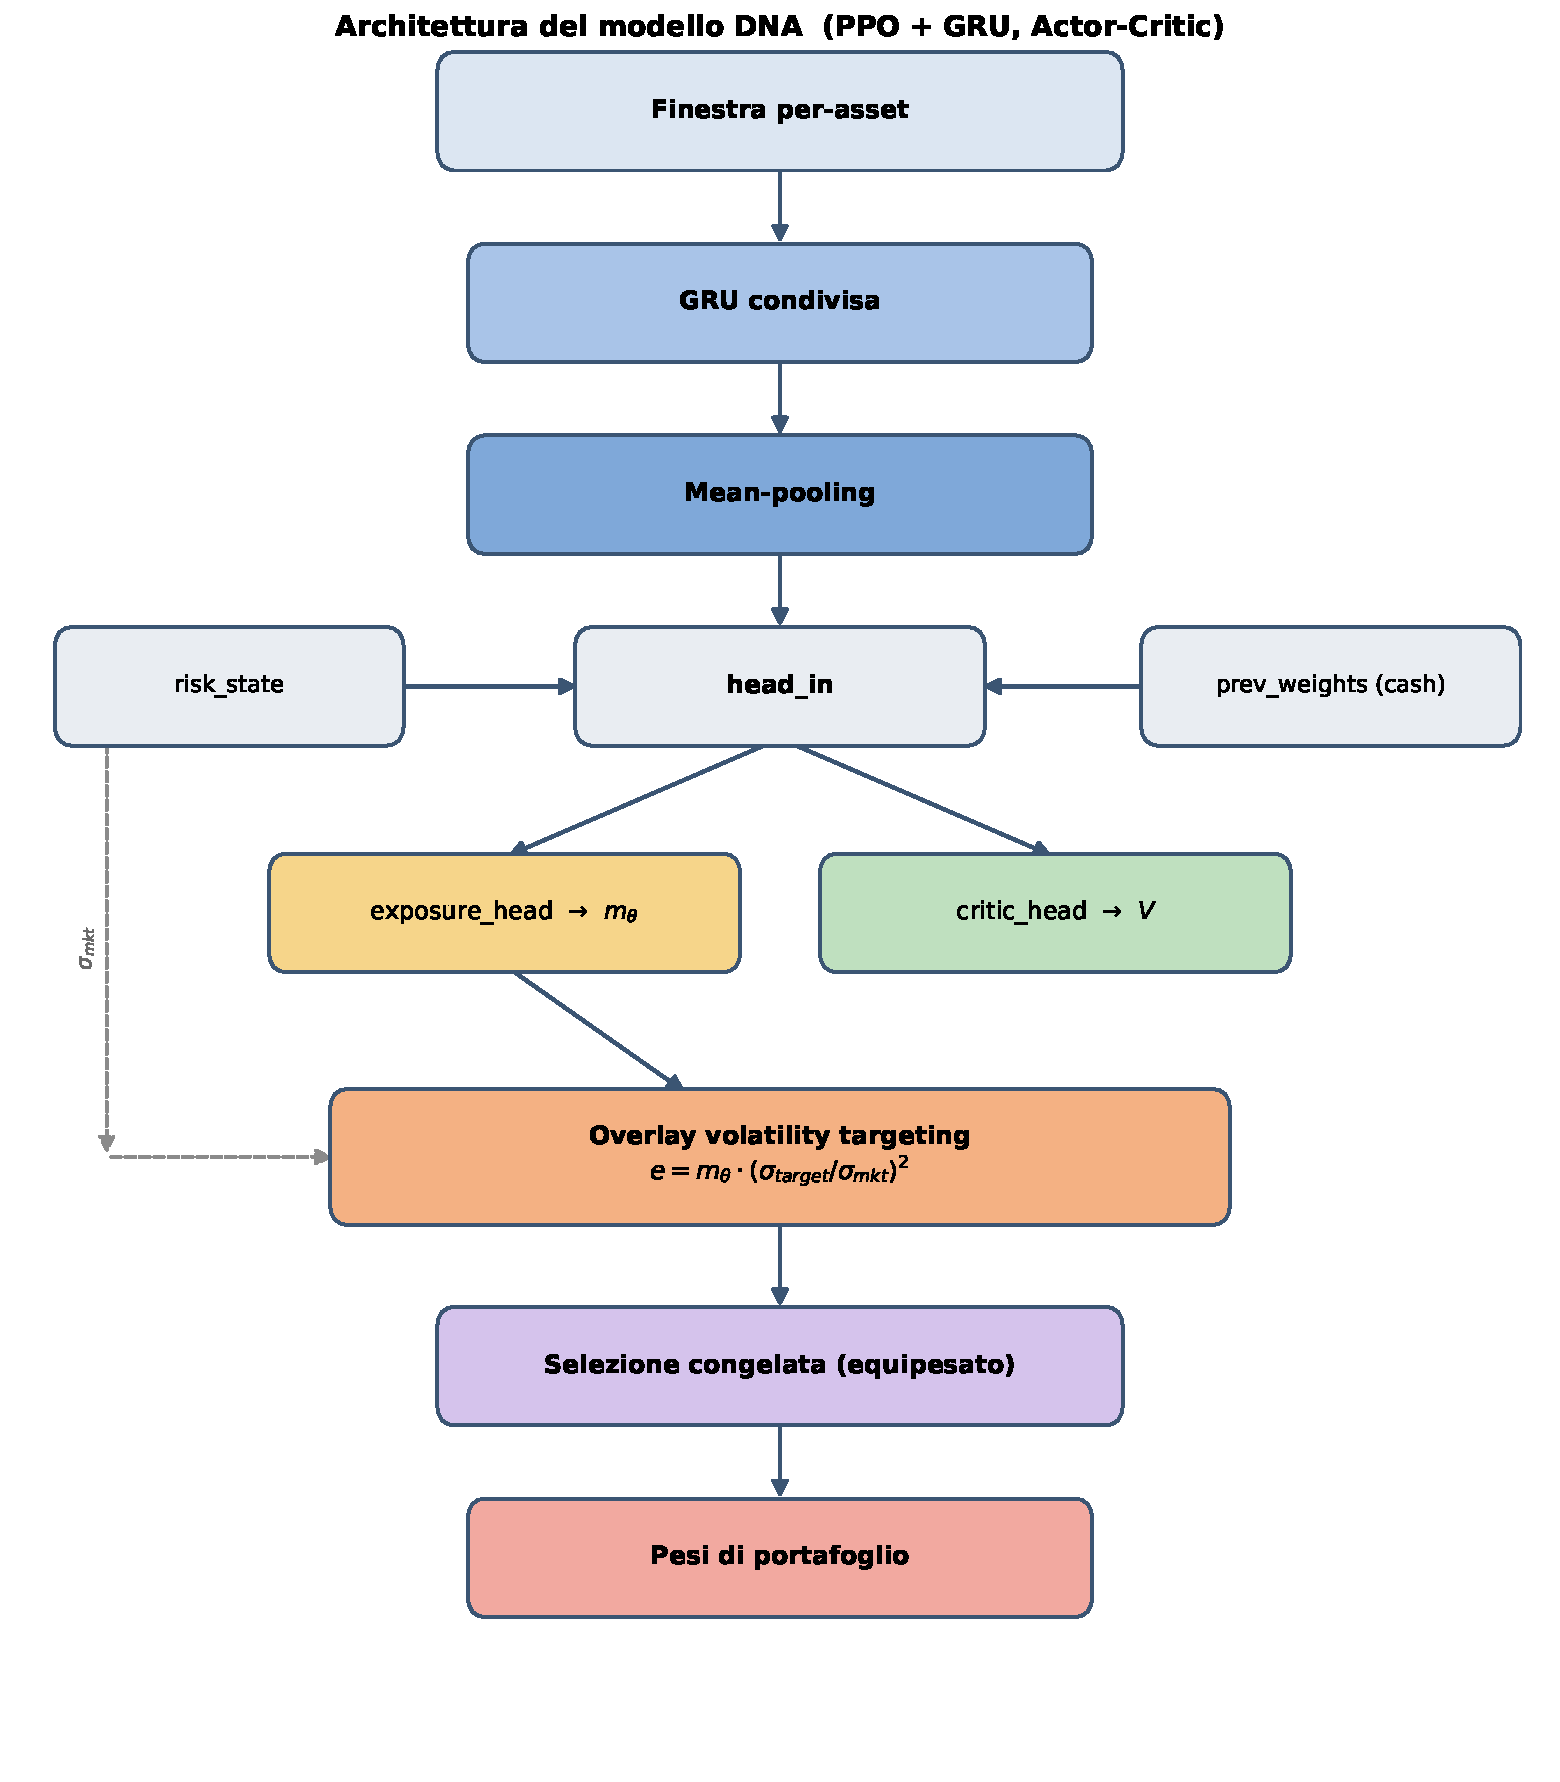
\includegraphics[width=0.8\textwidth]{architettura.pdf}
\caption{Architettura del modello: dalla finestra per-asset, tramite GRU condivisa e mean-pooling, al vettore \lstinline{head_in} (con \lstinline{risk_state} e \lstinline{prev_weights}), fino all'overlay di volatility targeting e ai pesi di portafoglio.}
\label{fig:architettura}
\end{figure}

Prima di effettuare qualunque operazione avviene la fase di normalizzazione descritta poco sopra, in seguito questi dati vengono passati alla GRU.
\paragraph{GRU}
Riceve features della forma $(B, N, 30, 4)$ e applica un reshape che fonde \textbf{B} e \textbf{N} in un'unica dimensione di taglia $B\times N$, usata come nuovo batch della GRU. In questo modo ogni asset di ogni campione diventa un esempio indipendente processato dalla stessa identica GRU: in sostanza c'è una sola GRU applicata a ciascuno degli $N$ asset.
La struttura interna della GRU è composta da 2 layer impilati, \lstinline{hidden_size=10}, \lstinline{batch_first=True}.
\begin{itemize}
  \item Layer 1: input 4 feature → 10 hidden.
  \item Layer 2: 10 → 10.
\end{itemize}
 
Si prende in seguito solo l'ultimo timestep ovvero un vettore di 10 elementi contenente una sintesi appresa della dinamica recente dell'asset. 
Ora abbiamo un embedding per ogni asset, poiché la stessa rete è applicata a ciascun asset in modo indipendente, l'embedding di ciascuno dipende solo dalla sua serie storica, non da chi gli sta accanto nè dalla sua posizione nella lista. 
Quindi scambiando due asset in input gli embedding si spostano insieme ai loro asset. 
È ancora presente l'equivarianza.
Dopo aver ottenuto gli embedding ne calcoliamo la media per ottenere il contesto di mercato.
\begin{lstlisting}[language=Typescript]
context = last_hidden.mean(dim=1)
\end{lstlisting}
La media è un'operazione simmetrica quindi il \lstinline{context} sarà identico qualunque sia l'ordine degli asset in questo modo otteniamo l'invarianza. 
L'invarianza ci permette di utilizzare il modello su qualsiasi asset non solo quelli su cui è stato addestrato. 
Anche se la media ci fa perdere la capacità di distinguere i singoli asset possiamo usarla in quanto, decidere quanto esporsi al mercato è una proprietà del portafoglio nel suo insieme e non deve dipendere da un'ordinamento arbitrario

\paragraph{Actor}
Nel modello l'Actor non si occupa di scegliere direttamente l'esposizione, ma produce un unico moltiplicatorre appreso $m_\theta$ che andrà poi a correggere una formula fissa di volatility targeting. 
Riceve in input un vettore da 17 elementi, ottenuto concatenando il contesto di mercato (i 10 numeri in output della GRU), il \lstinline{risk_state} del portafoglio e la quota di cash attuale:

\begin{lstlisting}[language=Typescript, caption={Struttura della testa di esposizione}]
exposure_head = Sequential(
    Linear(17 -> 16), ReLU, Linear(16 -> 1)
)
m_theta = softplus(exposure_head(input))   # m_theta > 0
\end{lstlisting}

L'output della exposure head passa poi in una \lstinline{softplus} che garantisce $m_\theta > 0$.
Il bias dell'ultimo layer è inizializzato in modo che al passo zero $\text{softplus}(\text{bias})=1$. 
Quindi il modello parte con $m_\theta \approx 1$, cioè come volatility targeting puro. I pesi del layer sono inoltre scalati di un fattore $0.1$ in questo modo la parte da appredere cresce lentamente invece di dominare da subito con valori casuali. In sostanza l'unico grado di libertà appreso della decisione è una correzzione moltiplicativa attorno a $1$ sopra una regola deterministica.

\paragraph{Overlay di volatility targeting}
È il componente che trasforma il moltiplicatore appreso $m_\theta$ nella decisione di esposizione $e_t$, applicando la formula di volatility targeting descritta nella metodologia (Sez.~\ref{sec:metodi}). 
Una volta ottenuta $e_t$ la selezione degli aset è congelata a equal weight e la liquidità riceve $1- e_t$.
L'ordine con cui elenchiamo i titoli non conta. Infatti se invertiamo la posizione di due asset all'ingresso del modello, anche i rispettivi pesi in uscita si scambieranno di posto, senza alterare la decisione finale.

\paragraph{Critic}
Il Critic serve unicamente durante l'addestramento come baseline per il calcolo del vantaggio in PPO.
Fornisce all'algoritmo PPO una stima del valore dello stato che serve a rendere l'apprendimento più stabile. 
Ha la stessa struttura della \lstinline{exposure_head} e riceve lo stesso identico input da 17 elementi:
\begin{lstlisting}[language=Typescript, caption={Struttura del critic}]
critic_head = Sequential(
    Linear(17 -> 16), ReLU, Linear(16 -> 1)
)
\end{lstlisting}

L'output è un singolo scalare $V(s)$ che rappresenta la stima del ritorno atteso a partire dallo stato corrente. 
Questo valore viene usato da PPO come baseline nel calcolo del vantaggio: invece di aggiornare la policy in base al ritorno grezzo $R_t$ si usa infatti il vantaggio $A_t = R_t - V(s_t)$ che misura quanto meglio del previsto è andata l'azione. 
Sottrare $V(s_t)$ riduce la varianza del gradiente e quindi rende l'addestramento più stabile e veloce. 

\paragraph{Output del modello}
Il modello restituisce in output il vettore dei pesi di portafoglio \[
w = \big[\, \underbrace{e_t/(N-1),\ \dots,\ e_t/(N-1)}_{N-1\ \text{asset rischiosi}},\ \underbrace{1 - e_t}_{\text{cash}} \,\big],
\] dove $e_t$ è l'esposizione prodotta dall'overlay vol targeting. È una distribuzione che somma a 1, con ultimo elemento la liquidità e gli asset tutti allo stessto peso.

\subsection{Environment}
L'ambiente \lstinline{PortfolioEnv} implementa la simulazione di mercato con cui l'agente interagisce. 
A ogni step (un giorno di borsa) gli fornisce un'osservazione, riceve un'azione, esegue il ribilanciamento tenendo conto dei costi, fa evolvere il valore del portafoglio e calcola la ricompensa.


Lo stato che l'agente riceve a ogni step è composto da tre elementi:
\begin{itemize}
    \item \textbf{feature di mercato} per ogni asset (la finestra di 30
    giorni di \lstinline{high, low, close, vix}), che passano per la GRU;
    \item \textbf{pesi correnti} del portafoglio \lstinline{prev_weights};
    \item \textbf{stato di rischio} \lstinline{risk_state}, sei scalari
    globali (uguali per tutti gli asset) che descrivono la salute del portafoglio e il regime di
    mercato.
\end{itemize}
La volatilità e il tempo in drawdown sono compresse con $\log(1+x)$ per fare in modo che pochi eventi estremi non possano pesare troppo nell'osservazione, il drawdown resta lineare.


Una volta ricevuti i nuovi \lstinline{prev_weights} , l'ambiente li applica attraverso due passaggi. 
Prima calcola i costi di transazione legati al ribilanciamento, poi aggiorna il valore del portafoglio applicando i prezzi di mercato del giorno corrente.
Da questo ricalcolo si ricavano il rendimento giornaliero, il nuovo massimo storico raggiunto e il drawdown attuale. 
Infine, la volatilità di mercato impiegata nel \lstinline{risk_state} e nell'overlay non è una variabile esterna fornita dal dataset, ma un segnale calcolato internamente. 
Essa è la deviazione standard mobile dei rendimenti a 21 giorni del paniere equipesato, riscalata su base annua ($\times\sqrt{252}$).

\paragraph{Costi di transazione (\lstinline{TransactionOptimizer})}
Nella realtà ogni operazione di mercato prevede il pagamento di commissioni.
Passare dalla composizione attuale del portafoglio $w'$ ai nuovi pesi desiderati $w$ richieda di comprare e vendere titoli.
Anche nell'ambiente simulato è stato fatto in modo che per ogni transazione si paghi una commissione dello $0{,}2\%$.
Questo costo viene quantificato tramite un fattore di rimanenza $\mu \in (0,1]$, che rappresenta la quota di capitale effettivamente intatta dopo aver pagato i costi: $V_{\text{post}} = \mu\, V_{\text{pre}}$. 
Il valore di $\mu$ è definito dall'equazione:\begin{equation}\mu = 1 - \sum_i \Big[\, b_i \max(\mu\,p_i - p'_i,\,0) + s_i \max(p'_i - \mu\,p_i,\,0)\,\Big],\end{equation}
dove $p_i$ e $p'_i$ sono le quote target e correnti del titolo $i$, mentre $b_i$ e $s_i$ indicano le commissioni per acquisti e vendite.
Il capitale finale $\mu$ dipende dal ricavo ottenuto vendendo i vari titoli a cui vengono sottratti i costi di commissione, l'ammontare delle commissioni però dipende a sua volta dal capitale finale.
Questo problema è stato risolto tramite una serie di iterazioni a punto fisso adottando lo schema proposto da Jiang et al.~\cite{jiang2017deep}. Anche nel modello originale della DNA~\cite{betancourt2021deep} sono applicati i costi di transazione, ma vengono calcolati attraverso un programma lineare (LP). 
Si è scelto di implementare i costi di transazione con un metodo di iterazione a punto fisso perché in questo modo è stato possibile trasferire il modello on-device nell'applicazione.
Includere questi costi impedisce alla rete di ottenere facili guadagni teorici attraverso un continuo ribilanciamento e garantisce che il risultato sia il più simile possibile a una situazione reale.

\paragraph{Episodio e ricompensa}
Un episodio non ha lunghezza fissa, esso parte
da un giorno estratto a caso e prosegue fino all'ultimo giorno del periodo di
addestramento. La durata varia quindi da un minimo
garantito di 252 giorni di borsa (circa un anno) fino all'intero orizzonte di training. 
A ogni passo l'ambiente restituisce la ricompensa, la cui
forma è discussa nella sezione sulla metodologia (Sez.~\ref{sec:metodi}).


\paragraph{Provenienza}
Il termine base di log-rendimento è la scelta standard nel portfolio management
con reinforcement learning . I due termini di penalità non derivano invece
da un singolo lavoro di letteratura, ma sono un reward shaping progettato
appositamente per questo modello: sono la traduzione, nella funzione obiettivo,
dell'idea che la difesa debba attivarsi quando il rischio di mercato aumenta.
L'overlay su cui la reward agisce è a sua volta l'analogo appreso del volatility
targeting~\cite{moreira2017volatility}.

\subsection{Addestramento}
Il modello è stato addestrato con \textbf{Proximal Policy Optimizaton} (PPO), un algoritmo di reinforcement learning on-policy della famiglia Actor-Critic~\cite{schulman2017proximal}. L'addestramento alterna una fase di raccolta di esperienza ottenuta facendo interagire la policy corrente con l'ambiente, con il successivo aggiornamento dei pesi in base ai dati raccolti.

\paragraph{Algoritmo di addestramento (PPO)}
L'addestramento segue uno schema iterativo suddiviso in tre fasi:
\begin{enumerate}
    \item \textbf{Raccolta dell'esperienza:} a ogni ciclo, l'agente interagisce simultaneamente con \lstinline{n_envs} ambienti di mercato indipendenti, registrando una traiettoria di \lstinline{n_steps} passi temporali per ciascuno.

    \item \textbf{Valutazione delle decisioni (Advantage):} il vantaggio $A_t$ di ogni azione è stimato con la Generalized Advantage Estimation (GAE)~\cite{schulman2016gae}, ovvero lo scarto tra il rendimento ottenuto e quello previsto dal Critic (cfr. Cap.~\ref{chap:backgrounds}).

    \item \textbf{Aggiornamento prudente della policy:} i pesi sono aggiornati massimizzando l'obiettivo clippato di PPO, che limita l'ampiezza di ogni singolo aggiornamento e la divergenza della strategia (cfr. Cap.~\ref{chap:backgrounds}).
\end{enumerate}

La funzione di perdita complessiva combina la loss della policy con l'errore di stima del Critic (pesato dal coefficiente \lstinline{vf_coef}). 
L'ottimizzazione viene  eseguita con l'algoritmo Adam su minibatch, applicando un vincolo sul gradiente per impedire oscillazioni numeriche distruttive lungo le \lstinline{n_epochs} passate sui dati.
La catena che lega il tutto è: 
 
la reward si accumula nel ritorno $R_t$; il Critic prova a prevederlo con $V(s)$; la differenza è il vantaggio; il vantaggio entra nella loss che spinge l'Actor a ripetere le azioni con vantaggio positivo.

\paragraph{Esplorazione}
Dato che la selezione è congelata e l'unica decisione appresa è l'esposizione, PPO
esplora campionando solo l'esposizione da una distribuzione Beta.
La rete produce un valore di esposizione deterministico, la policy è la Beta centrata su quel valore, che permette all'agente di esplorare valori di esposizione vicini.
L'ampiezza dell'esplorazione è regolata da un parametro appreso $\kappa$, così la rete decide da sola quanto esplorare.
In inferenza il campionamento è rimosso: la policy diventa deterministica e coincide con l'esposizione prodotta dalla rete.

\paragraph{Dati e suddivisione temporale}
L'addestramento avviene su un paniere di 8 large-cap
(\lstinline{CAT DIS HD IBM JNJ JPM PG UNH}) con finestra di osservazione di 30
giorni. 
Sono stati scelti solo 8 titoli perché esperimenti preliminari hanno dimostrato che usare un paniere più ampio durante l'addestramento non migliora le performance ma rende il modello meno cauto nella geestione dell'esposizione. 
 I dati sono divisi cronologicamente per evitare qualsiasi lookahead:
addestramento sul periodo 2000--2012, validazione 2012--2015, e test fuori campione dal 2015 in poi. Grazie all'invarianza per permutazione e
all'N-agnosticismo, il modello allenato su questo paniere può poi essere valutato
zero-shot su universi diversi.

\paragraph{Iperparametri}
\begin{center}
\begin{tabular}{lc}
\toprule
Iperparametro & Valore \\
\midrule
Ambienti paralleli (\lstinline{n_envs})        & 8 \\
Passi per rollout (\lstinline{n_steps})        & 128 \\
Epoche per aggiornamento (\lstinline{n_epochs})& 5 \\
Dimensione minibatch                           & 256 \\
Passi totali di training                       & 700\,000 \\
Fattore di sconto $\gamma$                     & 0.9 \\
$\lambda$ della GAE                            & 0.95 \\
Raggio di clipping $\epsilon$                  & 0.2 \\
Peso value loss (\lstinline{vf_coef})          & 0.5 \\
Coeff. entropia (\lstinline{ent_coef})         & 0 \\
Learning rate (Adam)                           & $3\times10^{-4}$ \\
Norma massima del gradiente                    & 0.5 \\
Concentrazione iniziale $\kappa$               & 50 \\
\bottomrule
\end{tabular}
\end{center}


	\clearpage{\pagestyle{empty}\cleardoublepage}

   

    \chapter{Esperimenti e Risultati}
    \thispagestyle{chapterplain}
    \label{chap:esperimenti}
    % !TEX root = main.tex
\section{Conclusioni: cosa aggiunge l'apprendimento}
\label{sec:conclusioni-finale}
In questa parte andiamo a esporre i vari esperimenti fatti, mostrando i risultati ottenuti da questo modello. 

\subsection{Esperimento 1: Come influisce il parametro \texorpdfstring{$\sigma_{\mathrm{target}}$}{sigma target}} 
Congelando la parte appresa ($m_\theta=1$, Moreira--Muir pura) il profilo di
rischio non cambia. Sul periodo 2015/26 il modello appreso e la formula pura hanno
lo stesso massimo drawdown entro il rumore (MDD $0.185$ vs $0.219$) e un
Calmar confrontabile ($1.24$ vs $1.13$); la rete converge sistematicamente su
$m_\theta\approx 1$ riproducendo in sostanza la regola deterministica. 

Confrontando varie versioni del modello che differiscono per il parametro $\sigma_{\mathrm{target}}$, cioè la volatilità annuale del portafoglio che
il modello cerca di mantenere, capiamo che cambiare questa variabile non porta a dei miglioramenti. 
$\sigma_{\mathrm{target}}$ è la manopola che abbiamo sul drawdown, aumentando il suo valore aumenta anche il massimo drawdown ottenuto in modo monotono, 
insomma è il parametro che ci permette di scegliere il rischio di perdita che vogliamo avere e non porta a nessun tipo di ottimizzazione dell'apprendimento.

\begin{table}[H]
\centering
\small
\caption{Esperimento 1 --- overlay appreso ($m_\theta$) vs formula
pura ($m_\theta{=}1$, Moreira--Muir) ai vari $\sigma_{\mathrm{target}}$, periodo
2015--2026 (mediana su 3 seed).}
\label{tab:exp1-mm-sweep}
\begin{tabular}{llcccc}
\toprule
$\sigma_{\mathrm{target}}$ & Overlay & cash & MDD & Calmar & Sharpe \\
\midrule
\multirow{2}{*}{0.10}
 & appreso ($m_\theta$)     & 0.790 & 0.056 & 0.85 & 1.115 \\
 & formula ($m_\theta{=}1$) & 0.615 & 0.089 & 1.04 & 1.240 \\
\midrule
\multirow{2}{*}{0.15}
 & appreso ($m_\theta$)     & 0.438 & 0.105 & 1.35 & 1.361 \\
 & formula ($m_\theta{=}1$) & 0.337 & 0.138 & 1.35 & 1.442 \\
\midrule
\multirow{2}{*}{0.20}
 & appreso ($m_\theta$)     & 0.217 & 0.185 & 1.24 & 1.466 \\
 & formula ($m_\theta{=}1$) & 0.179 & 0.219 & 1.13 & 1.471 \\
\bottomrule
\end{tabular}
\end{table}


\paragraph{Conservatività, non intelligenza.} 
Per capire se la rete neurale abbia davvero sviluppato una capacità di prevedere quando uscire dal mercato prima dei crolli, è necessario separare l'effetto del tempismo da quello del livello medio di liquidità mantenuto. 
Per farlo abbiamo tracciato una frontiera di controllo. Abbiamo preso un piano cartesiano dove l'asse x contiene il livello di cash medio mantenuto mentre l'asse y contiene l'MDD. 
Su questo piano cartesiano viene tracciata una curva che unisce le varie collocazioni della formula di volatility targeting di Moreira e Muir al variare di $\sigma_{\mathrm{target}}$. Se l'agente avesse appreso un'intelligenza predittiva superiore, dovrebbe posizionarsi al di sotto di questa curva: a parità di liquidità media, dovrebbe cioè subire perdite massime inferiori grazie alla tempestività dei suoi interventi.
(Fig.~\ref{fig:frontier}). 

I dati mostrano invece l'esatto contrario: \textbf{il modello appreso cade esattamente sulla frontiera della formula deterministica} in tutti i cinque regimi di mercato considerati. 
Gli scarti di MDD sono trascurabili e privi di un pattern sistematico. 
Questo dimostra che il drawdown minore ottenuto dal modello rispetto alla formula standard allo stesso $\sigma_{\mathrm{target}}$ non deriva da una gestione dinamica intelligente, ma semplicemente dal fatto che l'agente sceglie di rimanere mediamente più disinvestito. 
Si tratta di pura conservatività: lo stesso identico livello di protezione si può ottenere con la formula statica, limitandosi ad abbassare il bersaglio di volatilità.



\begin{figure}[H]
\centering
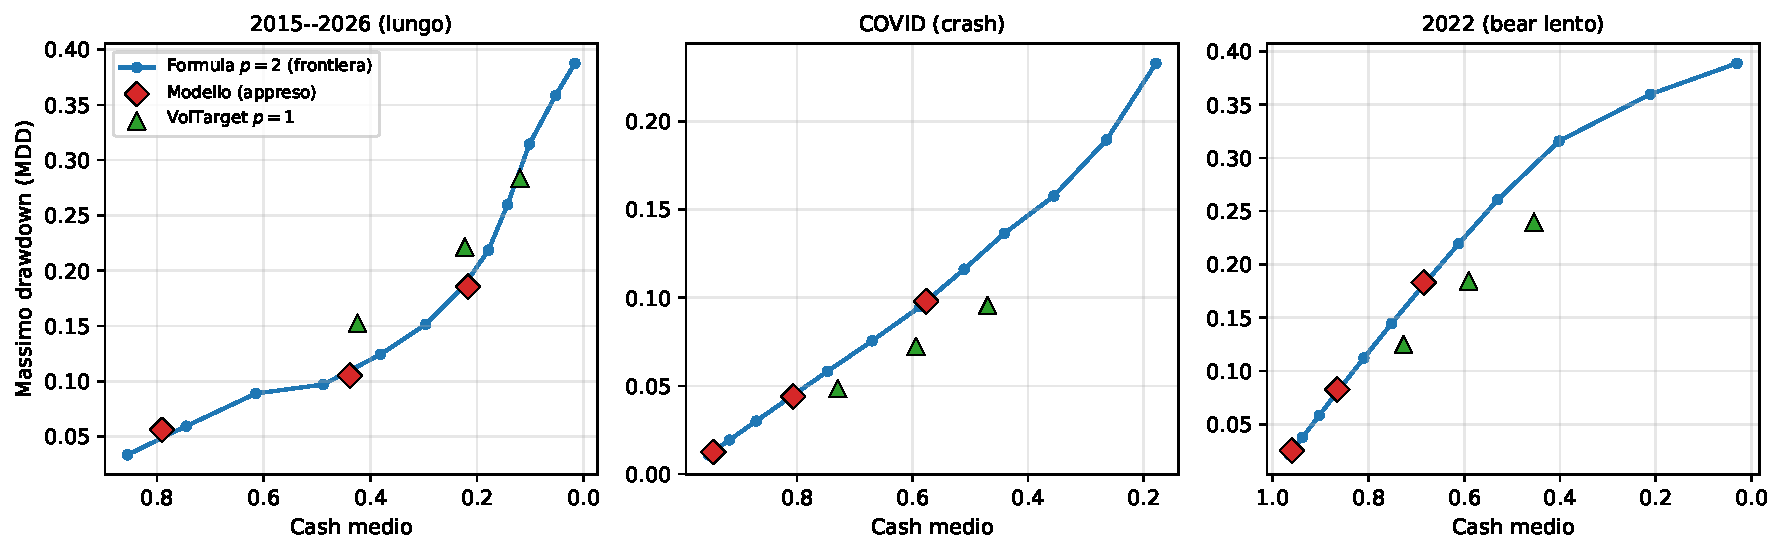
\includegraphics[width=\textwidth]{frontier_mdd.pdf}
\caption{Frontiera cash medio--MDD. Curva blu: formula fissa ($p=2$, $m_\theta=1$) al variare di $\sigma_{\mathrm{target}}$; rombi rossi: modello appreso ($\sigma_{\mathrm{target}}=0.10,\,0.15,\,0.20$); triangoli verdi: volatility targeting classico ($p=1$), stessi $\sigma_{\mathrm{target}}$.}
\label{fig:frontier}
\end{figure}



\begin{table}[H]
\centering
\caption{Confronto a $\sigma_{\mathrm{target}}=0.20$ delle quattro strategie
(mediana su 3 seed). ``modello'' $=m_\theta$ appreso; ``formula'' $=$ Moreira--Muir
pura ($p=2$); ``voltarget'' $=$ volatility targeting classico ($p=1$);
``equipesato'' $=$ paniere equipesato pienamente investito.}
\label{tab:exp1-strategie}
\begin{tabular}{llccc}
\toprule
Periodo & Strategia & MDD & Calmar & Sharpe \\
\midrule
\multirow{4}{*}{2015--26}
 & modello    & $0.185$ & $1.24$  & $1.47$ \\
 & formula    & $0.219$ & $1.13$  & $1.47$ \\
 & voltarget  & $0.284$ & $0.96$  & $1.44$ \\
 & equipesato & $0.379$ & $0.80$  & $1.25$ \\
\midrule
\multirow{4}{*}{COVID}
 & modello    & $0.098$ & $4.17$  & $2.47$ \\
 & formula    & $0.116$ & $4.05$  & $2.47$ \\
 & voltarget  & $0.096$ & $7.20$  & $2.83$ \\
 & equipesato & $0.323$ & $2.99$  & $1.71$ \\
\midrule
\multirow{4}{*}{2022}
 & modello    & $0.183$ & $-0.95$ & $-1.62$ \\
 & formula    & $0.219$ & $-0.95$ & $-1.60$ \\
 & voltarget  & $0.240$ & $-0.91$ & $-1.13$ \\
 & equipesato & $0.379$ & $-0.95$ & $-1.15$ \\
\midrule
\multirow{4}{*}{2025}
 & modello    & $0.153$ & $0.94$  & $0.98$ \\
 & formula    & $0.165$ & $0.92$  & $0.98$ \\
 & voltarget  & $0.100$ & $3.54$  & $1.95$ \\
 & equipesato & $0.227$ & $1.13$  & $1.08$ \\
\bottomrule
\end{tabular}
\end{table}

\begin{figure}[H]
\centering
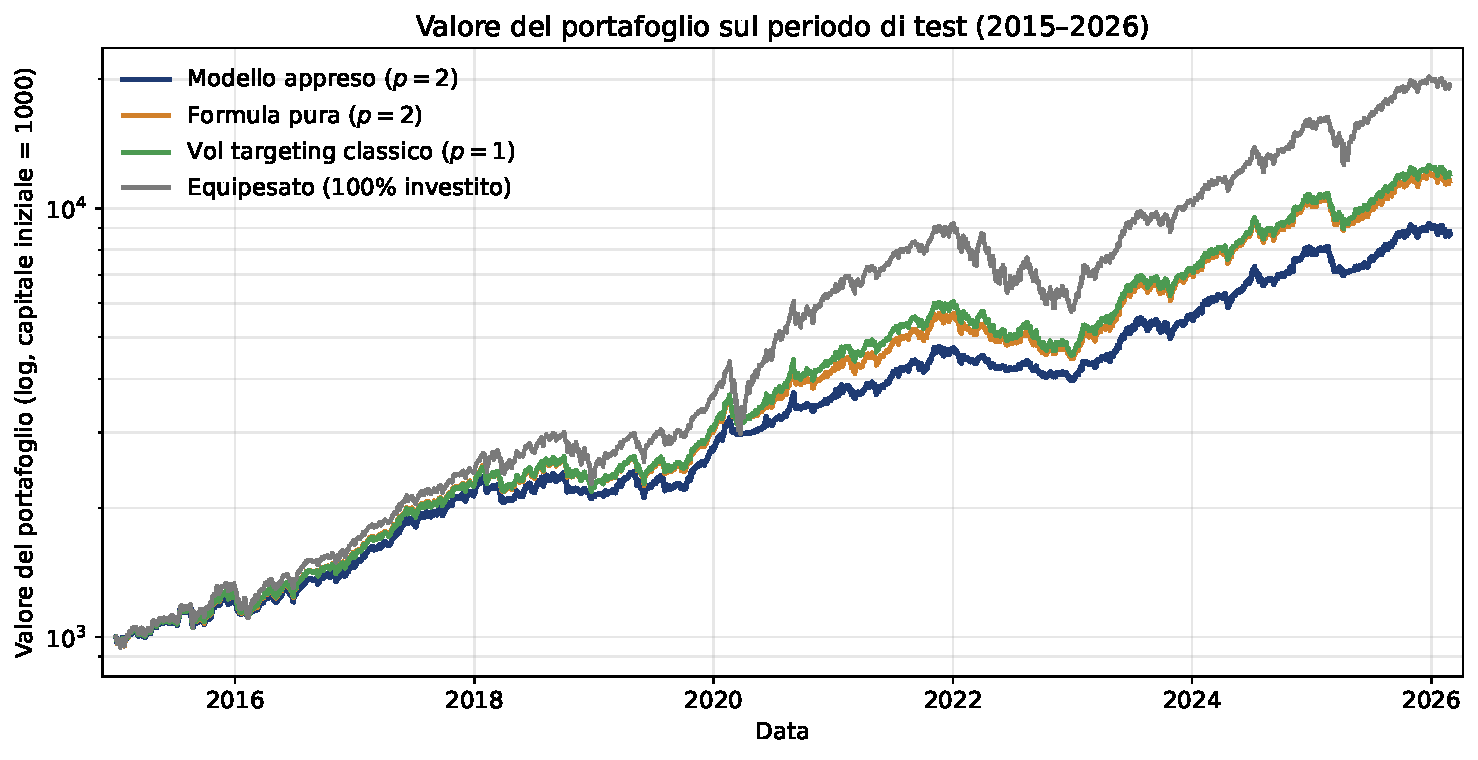
\includegraphics[width=\textwidth]{equity_curve.pdf}
\caption{Valore del portafoglio nel tempo sul periodo di test (2015--2026): modello appreso, formula pura ($p=2$), volatility targeting classico ($p=1$) ed equipesato pienamente investito.}
\label{fig:equity-curve}
\end{figure}


\subsection{Esperimento 2: L'esponente al centro delle osservazioni}

Dai risultati dello scorso esperimento abbiamo visto che il valore dell'esponente può fare la differenza in alcuni momenti del mercato grazie alla velocità e grandezza della reazione ai periodi di turbolenza, questa osservazione ci porta direttamente all'esperimento numero due.
Quando l'esponente della formula è mantenuto fisso, il valore di $p$ funge da principale leva difensiva, ma la sua efficacia dipende fortemente dal tipo di mercato:
\begin{itemize}
\item Nei crolli improvvisi e violenti (come il crash COVID del 2020 o il sell-off dei dazi del 2025) l'esponente $p=1$ si comporta meglio. 
Questo perché riducendo l'esposizione in modo più moderato evita un'uscita eccessiva che farebbe perdere il rimbalzo successivo. 
Il vantaggio è evidente soprattutto sul rendimento corretto per il rischio (Sharpe e Calmar più alti), in quanto la strategia restando parzialmente investita partecipa alla ripresa del mercato.
\item Nei ribassi lenti e prolungati (come il bear market del 2022) e sull'orizzonte storico di lungo periodo, un esponente $p=2$ contiene meglio il drawdown. 
Quando la volatilità sale, anche in modo moderato ma persistente, la reazione amplificata dal quadrato riduce la quota investita in maniera più decisa, mantenendo più liquidità.
\end{itemize}
Nessun valore fisso, dunque, riesce a dominare su tutti i contesti di mercato.


Da questa constatazione abbiamo sviluppato due esperimenti paralleli:
\begin{itemize}
    \item Rendere l'esponente $p$ apprendibile dalla rete.
    \item Imporre una regola fissa che scambia il modello dalla versione con $p=1$ a quella con $p=2$ quando vengono superati determinati limiti.
\end{itemize}

\subsubsection{Esponente appreso}
Partendo dall'ipotesi che lasciar apprendere l'esponente alla rete neurale possa permettergli di adattarsi dinamicamente al contesto si è sviluppato il seguente esperimento.

Prima di tutto la rete è stata modificata aggiungendo una nuova \lstinline{exposure_head} che si concentra sul calcolare l'esponente.
Questa testa lavora in parallelo con quella progettata per l'esposizione.
Per prendere la decisione utilizza gli stessi dati dell'altra che decide l'esposizione e ottimizza la stessa reward.
La nuova testa può decidere valori dell'esponente compresi tra 1 e 2 e la sua scelta segue una funzione Sigmoidea.

Andiamo ora a osservare risultati dell'esperimento:
\begin{itemize}
    \item \textbf{Sul fronte del rendimento corretto per il rischio (Sharpe ratio):} il modello con esponente appreso si dimostra inferiore. Le sue prestazioni restano sempre a metà strada tra $p=1$ e $p=2$.
    \item \textbf{Sul fronte della pura protezione dalle perdite (Drawdown):} a una prima lettura sembrerebbe un successo. Sul periodo 2015--2026, l'esponente appreso registra un MDD più contenuto e un Calmar ratio più elevato di entrambe le formule fisse. Questo potrebbe far pensare che l'agente abbia imparato a dosare la leva difensiva meglio delle regole statiche.
\end{itemize}

Ripetendo però lo stesso controllo di frontiera visto nell'Esperimento~1, questo presunto vantaggio svanisce. La minore perdita non nasce da una reale intelligenza di contesto, ma dal fatto che il modello si posiziona su un livello di liquidità media più alto di entrambe le regole a confronto. 

A parità di capitale medio investito, le prestazioni del modello tornano a ricadere esattamente sulla frontiera deterministica (Fig.~\ref{fig:frontier}). Lo stesso identico livello di protezione è perfettamente replicabile abbassando il parametro $\sigma_{\mathrm{target}}$ della formula fissa.

In conclusione, anche sul drawdown, la metrica specifica per cui era stato ottimizzato, l'esponente appreso non aggiunge nulla che una configurazione strutturale leggermente più conservativa non offra già a costo zero. L'efficacia della protezione risiede interamente nelle scelte a monte dell'architettura, non nei pesi dinamici appresi dalla rete.

\begin{table}[H]
\centering
\small
\caption{Esperimento 2: esponente $p$ dell'overlay a confronto
(\texttt{DD\_VOL\_PENALTY}, $\sigma_{\mathrm{target}}=0.20$, mediana su 3 seed).
$p=1$ vol targeting, $p=2$ variance targeting, $p$ appreso regime-dipendente.}
\label{tab:exp2-esponente}
\begin{tabular}{llccccccc}
\toprule
Periodo & Esponente & cash & MDD & Calmar & Sharpe \\
\midrule
\multirow{4}{*}{2015--26}
 & $p=1$      & $0.155$ & $0.251$ & $1.00$ & $1.430$ \\
 & $p=1.5$    & $0.239$ & $0.191$ & $1.16$ & $1.456$ \\
 & $p=2$      & $0.220$ & $0.184$ & $1.24$ & $1.463$ \\
 & appreso    & $0.229$ & $0.164$ & $1.39$ & $1.447$ \\
\midrule
\multirow{4}{*}{COVID}
 & $p=1$      & $0.431$ & $0.153$ & $3.41$ & $2.280$ \\
 & $p=1.5$    & $0.584$ & $0.102$ & $3.76$ & $2.438$ \\
 & $p=2$      & $0.579$ & $0.097$ & $4.18$ & $2.477$ \\
 & appreso    & $0.612$ & $0.085$ & $4.61$ & $2.470$ \\
\midrule
\multirow{4}{*}{2022}
 & $p=1$      & $0.476$ & $0.252$ & $-0.95$ & $-1.417$ \\
 & $p=1.5$    & $0.650$ & $0.187$ & $-0.95$ & $-1.520$ \\
 & $p=2$      & $0.688$ & $0.181$ & $-0.95$ & $-1.616$ \\
 & appreso    & $0.757$ & $0.162$ & $-0.96$ & $-1.736$ \\
\midrule
\multirow{4}{*}{2017}
 & $p=1$      & $0.005$ & $0.047$ & $9.67$ & $3.132$ \\
 & $p=1.5$    & $0.007$ & $0.047$ & $9.68$ & $3.122$ \\
 & $p=2$      & $0.005$ & $0.047$ & $9.67$ & $3.132$ \\
 & appreso    & $0.005$ & $0.047$ & $9.67$ & $3.132$ \\
\midrule
\multirow{4}{*}{2025}
 & $p=1$      & $0.129$ & $0.174$ & $0.99$ & $1.038$ \\
 & $p=1.5$    & $0.191$ & $0.148$ & $0.99$ & $1.022$ \\
 & $p=2$      & $0.173$ & $0.152$ & $0.95$ & $0.984$ \\
 & appreso    & $0.178$ & $0.149$ & $0.96$ & $0.932$ \\
\bottomrule
\end{tabular}
\end{table}

\paragraph{Una loss dedicata all'esponente}

Dall'esperimento di sopra abbiamo dimostrato che utilizzando la stessa reward dell'esposizione non riusciamo a battere un esponente fisso.
Non essendo la reward specificatamente progettata per l'esponente ci si è chiesto se implementare una loss dedicata potrebbe portare a dei risultati vincenti.
In questo esperimento si è provato ad utilizzare una loss progettata specificatamente per addestrare la testa che decide l'esponente a prevedere quando la volatilità futura darà vita a un crollo.
In sostanza se la testa prevede un crollo imposta l'esponente $p=2$ altrimenti a $p=1$.

Per questo specifico problema si parla di apprendimento supervisionato.
È stata costruita un'etichetta che vale 1 quando il mercato scende di oltre il 10\% nei 21 giorni successivi, ovvero avviene un crollo, e 0 altrimenti.
La testa produce una probabilità di crollo prevista $\widehat{P}(\text{crollo})=\sigma(z)\in(0,1)$.
La loss usata per questo esperimento è una cross-entropy binaria (BCE).   
Ad ogni step la funzione di loss misura quanto la previsione del modello è distante dalla verità.
Penalizza di più in relazione a quanto il modello è sicuro di una previsione errata, cercando di spingere il modello a fare la previsione giusta.
La probabilità di crollo prevista infine viene sommata a uno per ricavare l'esponente finale $p = 1 + \widehat{P}(\text{crollo})$. 

Ancora prima di guardare i risultati dei backtest è venuto alla luce un altro problema: la loss va in stallo (Fig.~\ref{fig:regime-loss}).
All'inizio dell'addestramento la loss sembrava funzionare e l'errore scendeva gradualmente in modo corretto. 
Arrivati circa a metà la loss si è fermata ad un valore alto, vicino a quello di un predittore privo di informazione.
Dall'inizio dello stallo in poi la loss ha continuato ad oscillare sempre attorno allo stesso valore, a causa del rumore dei vari mini-batch, e scendendo di un valore irrisorio fino alla fine dell'addestramento.
Questo è avvenuto perché il modello ha raggiunto un tetto informativo, cioè partendo dai dati non gli è stato possibile estrarre l'informazione sulla direzione del mercato. 
Senza informazione direzionale non gli è stato possibile distinguere un crollo in arrivo da un semplice ribasso lento del mercato e questo lo ha portato nello stallo.

Dai backtest (Tab.~\ref{tab:exp-regime}) si mostra come la variante supervisionata non batte né l'esponente
appreso dal solo reward né la formula fissa $p=2$: presenta anzi un MDD più alto
in ogni periodo, tenendo meno cash, senza guadagno su Calmar o Sharpe.


\begin{figure}[H]
\centering
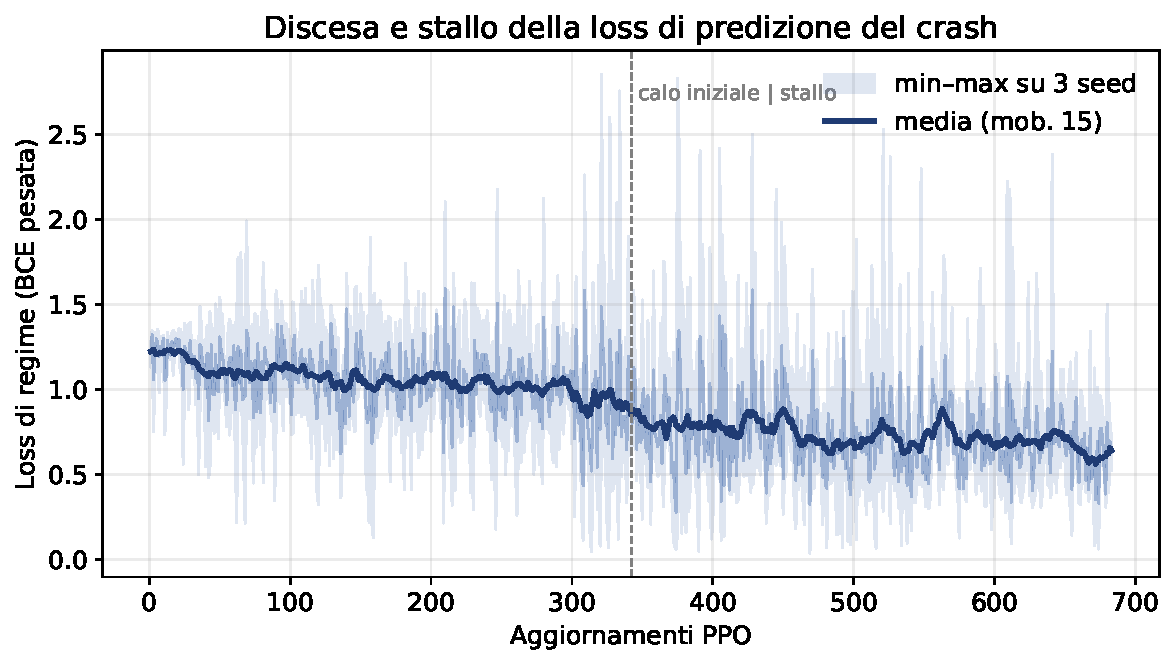
\includegraphics[width=0.8\linewidth]{regime_loss.pdf}
\caption{Loss BCE di predizione del crash durante l'addestramento (media su 3
seed, banda min--max).}
\label{fig:regime-loss}
\end{figure}

\begin{table}[H]
\centering
\small
\caption{Esponente con loss di regime (BCE) vs esponente appreso dal solo reward
(Esp.~2) vs formula fissa $p=2$, universo large-cap (mediana su 3 seed).}
\label{tab:exp-regime}
\begin{tabular}{llcccc}
\toprule
Periodo & Strategia & cash & MDD & Calmar & Sharpe \\
\midrule
\multirow{3}{*}{2015--26}
 & formula $p{=}2$      & $0.34$ & $0.138$ & $1.35$ & $1.44$ \\
 & appreso (reward)     & $0.37$ & $0.122$ & $1.41$ & $1.42$ \\
 & appreso + BCE        & $0.31$ & $0.166$ & $1.20$ & $1.44$ \\
\midrule
\multirow{3}{*}{COVID}
 & formula $p{=}2$      & $0.71$ & $0.067$ & $4.13$ & $2.52$ \\
 & appreso (reward)     & $0.74$ & $0.059$ & $4.06$ & $2.50$ \\
 & appreso + BCE        & $0.63$ & $0.090$ & $3.49$ & $2.32$ \\
\midrule
\multirow{3}{*}{2022}
 & formula $p{=}2$      & $0.78$ & $0.128$ & $-0.95$ & $-1.60$ \\
 & appreso (reward)     & $0.81$ & $0.111$ & $-0.95$ & $-1.61$ \\
 & appreso + BCE        & $0.68$ & $0.155$ & $-0.95$ & $-1.50$ \\
\midrule
\multirow{3}{*}{2025}
 & formula $p{=}2$      & $0.27$ & $0.119$ & $1.16$ & $1.09$ \\
 & appreso (reward)     & $0.31$ & $0.111$ & $1.19$ & $1.10$ \\
 & appreso + BCE        & $0.27$ & $0.123$ & $1.09$ & $1.09$ \\
\bottomrule
\end{tabular}
\end{table}

In sintesi, fornire una supervisione esplicita all'esponente non cambia l'esito.
Il limite non è la modalità di addestramento
ma l'assenza nei dati di un segnale sfruttabile sulla direzione futura dei
rendimenti.



\subsubsection{Regolare l'esponente con una regola}
Dato le precedenti osservazioni abbiamo pensato di affidare la scelta su quale esponente usare a una regola fissa. 
Questo permette di adattare dinamicamente l'esponente in base alla volatilità di mercato. 
La regola implementata consiste nell'aumentare l’aggressività del taglio di esposizione, cioè l'esponente $p$, man mano che sale l’indice VIX.


Tuttavia, anche questa soluzione fallisce: la regola ibrida riesce a eguagliare o superare la miglior formula fissa in \textbf{al più uno scenario su cinque}, sia in termini di drawdown che di Sharpe ratio.

Ci sono tre ragioni principali per cui questa soluzione non funziona:
\begin{enumerate}
    \item \textbf{Il compromesso diluisce l'efficacia:} variare $p$ in modo progressivo crea un'esposizione intermedia che finisce per non essere ottimale in nessun contesto: taglia troppo poco nei crolli improvvisi e troppo presto nelle fasi di lenta correzione.
    \item \textbf{Il VIX è un segnale reattivo, non predittivo:} il VIX non anticipa le crisi, ma esplode quando il crollo è già iniziato. Quando la regola rileva un picco di volatilità e decide finalmente di alzare l'esponente a $p=2$, la perdita di capitale si è già avvenuta in gran parte.
    \item \textbf{Asimmetria informativa:} capire se una discesa dei mercati sia l'inizio di un ribasso prolungato (dove servirebbe $p=1$) o di uno shock istantaneo (dove servirebbe $p=2$) è possibile solo a posteriori, mai in tempo reale mentre il fenomeno sta avvenendo.
\end{enumerate}

Quindi, un sistema difensivo basato su un segnale che arriva tardi non può impedire il danno. 
È come chiudere la porta dopo che il ladro è entrato. 
Il meccanismo di difesa si attiva, ma ormai i danni sono fatti.

\begin{table}[H]
\centering
\small
\caption{Esperimento 3: regola morbida sul VIX ($p:1\!\to\!2$ via
sigmoide) contro $p=1$ e $p=2$ fissi, in inferenza dallo stesso checkpoint
($\sigma_{\mathrm{target}}=0.20$, mediana su 3 seed).}
\label{tab:exp3-regola}
\begin{tabular}{llccccccc}
\toprule
Periodo & Modalita' & cash & MDD & Calmar & Sharpe \\
\midrule
\multirow{3}{*}{2015--26}
 & $p=1$ fisso  & $0.171$ & $0.240$ & $1.02$ & $1.433$ \\
 & $p=2$ fisso  & $0.220$ & $0.184$ & $1.24$  & $1.463$ \\
 & regola VIX   & $0.183$ & $0.234$ & $1.01$ & $1.432$ \\
\midrule
\multirow{3}{*}{COVID}
 & $p=1$ fisso  & $0.451$ & $0.148$ & $3.41$ & $2.281$ \\
 & $p=2$ fisso  & $0.579$ & $0.097$ & $4.18$ & $2.477$ \\
 & regola VIX   & $0.510$ & $0.122$ & $3.62$ & $2.380$ \\
\midrule
\multirow{3}{*}{2022}
 & $p=1$ fisso  & $0.504$ & $0.240$ & $-0.95$ & $-1.421$ \\
 & $p=2$ fisso  & $0.688$ & $0.181$ & $-0.95$ & $-1.616$ \\
 & regola VIX   & $0.550$ & $0.235$ & $-0.95$ & $-1.534$ \\
\midrule
\multirow{3}{*}{2017}
 & $p=1$ fisso  & $0.005$ & $0.047$ & $9.67$ & $3.129$ \\
 & $p=2$ fisso  & $0.005$ & $0.047$ & $9.67$ & $3.132$ \\
 & regola VIX   & $0.005$ & $0.047$ & $9.67$ & $3.130$ \\
\midrule
\multirow{3}{*}{2025}
 & $p=1$ fisso  & $0.140$ & $0.171$ & $1.00$ & $1.048$ \\
 & $p=2$ fisso  & $0.173$ & $0.152$ & $0.95$ & $0.984$ \\
 & regola VIX   & $0.149$ & $0.165$ & $0.90$ & $0.982$ \\
\bottomrule
\end{tabular}
\end{table}


\subsection{Generalità: trasferimento su panieri diversi}

Per verificare se im modello abbia davvero la proprietà di generalità o se sia invece legato al paniere azionario su cui è stata addestrato, abbiamo fatto un test di trasferimento. Abbiamo applicato il modello direttamente a portafogli completamente nuovi, senza fargli vedere prima i dati e senza alcun ri-addestramento. 

Grazie alla sua architettura, il modello può gestire portafogli di qualsiasi dimensione e composizione. Lo abbiamo quindi messo alla prova su panieri dell'indice S\&P~500 molto eterogenei per volatilità, settore di appartenenza, numerosità ($N=5$ e $N=20$) e grado di correlazione interna.

Sul decennio 2015--2026 (Tab.~\ref{tab:baskets-longrun}), la capacità difensiva del modello dimostra di saper \textbf{generalizzare con successo}:
\begin{itemize}
    \item \textbf{Difesa attiva reale ($\mathrm{MDD\_gain} > 0$):} su tutti i sei panieri testati, il modello contiene la perdita massima meglio di una strategia passiva con identica liquidità media (cioé il MDD del modello è minore rispetto a una strategia che tiene una liquidità sempre pari alla media del modello dal 2015 al 2026). Si tratta quindi di una gestione dinamica che aggiunge valore concreto.
    \item \textbf{Reattività anticiclica ($\rho_{\text{cash,dd}} > 0$):} la correlazione positiva conferma che il modello alza la quota di contante ogni volta che il mercato comincia a crollare, a prescindere dal tipo di titoli in portafoglio.
    \item \textbf{Flessibilità sul numero di titoli:} il meccanismo funziona altrettanto bene sia con un paniere ristretto di sole 5 azioni (\emph{small5}) sia con uno più ampio di 20 (\emph{large20}). Inoltre, nel paniere ben diversificato e a bassa correlazione le prestazioni restano solide, eliminando la paura che mantenere fissi i titoli nel tempo penalizzasse la strategia.
\end{itemize}

Dai risultati emerge un vincolo strutturale: la difesa è simmetrica ($\text{down\_capt} \approx \text{up\_capt}$).
Il modello reagisce puramente alla volatilità complessiva del paniere a presciendere dal fatto che sia a rialzo o ribasso.
Non c'è quindi alcun tipo di previsione direzionale.

\begin{table}[H]
\centering
\caption{\textbf{Trasferimento sul periodo lungo (2015--2026).}
Modello finale ($p=2$, mediana su 3 seed) su panieri mai visti in addestramento.
$\mathrm{MDD\_gain}>0$: drawdown ridotto meglio di un cash fisso di pari entità media;
$\rho_{\text{cash,dd}}$: tendenza ad alzare il contante al peggiorare delle perdite.}
\label{tab:baskets-longrun}
\begin{tabular}{lcccccc}
\toprule
Paniere & MDD & Calmar & MDD\_gain & down/up capt & $\rho_{\text{cash,dd}}$ \\
\midrule
difensivi     & $0.150$ & $0.68$ & $+0.115$ & $0.92/0.92$ & $0.38$  \\
diversificato & $0.156$ & $0.84$ & $+0.165$ & $0.87/0.86$ & $0.69$  \\
large20       & $0.241$ & $0.85$ & $+0.059$ & $0.82/0.82$ & $0.65$  \\
small5        & $0.169$ & $0.81$ & $+0.165$ & $0.87/0.86$ & $0.71$ \\
ciclici       & $0.383$ & $0.16$ & $+0.109$ & $0.71/0.68$ & $0.65$ \\
growth        & $0.201$ & $0.95$ & $+0.150$ & $0.52/0.52$ & $0.59$ \\
\bottomrule
\end{tabular}
\end{table}

Il riscontro più significativo si vede dallo stress test nei regimi critici (Tab.~\ref{tab:baskets-stress}): insieme alla capacità difensiva, si trasferisce in modo identico anche il limite dell'approccio. 
\begin{itemize}
    \item \textbf{Nei crolli violenti e rapidi (Crash COVID 2020):} la volatilità esplode immediatamente facendo scattare subito i tagli di esposizione. Il modello ottiene una vittoria netta su ogni paniere ($\mathrm{MDD\_gain} > 0$ ovunque).
    \item \textbf{Nei mercati ribassisti lenti e logoranti (Bear market 2022):} il modello fallisce su tutti i panieri ($\mathrm{MDD\_gain} \le 0$). In questo scenario i prezzi scendono con costanza ma senza picchi clamorosi di volatilità. 
    Il modello quindi non riceve quei segnali che gli indicano quando ritirarsi dal mercato in maniera aggressiva. 
    Per questo tiene sempre la liquidità abbastanza alta ma non ha nessun timing utile da sfruttare finendo per far peggio di un null a cash costante.

\end{itemize}

Questo schema è esattamente lo stesso osservato sui dati di addestramento. 
Il fatto che compaia anche su panieri del tutto nuovi ne dimostra la natura universale: non è un'anomalia di un singolo set di azioni, ma una proprietà strutturale del volatility targeting.

\begin{table}[H]
\centering
\caption{Difesa nei regimi di stress, zero-shot (modello finale $p=2$, mediana su
3 seed).}
\label{tab:baskets-stress}
\begin{tabular}{lcc}
\toprule
Paniere & MDD\_gain (COVID) & MDD\_gain (2022) \\
\midrule
difensivi     & $+0.096$ & $-0.003$ \\
diversificato & $+0.056$ & $-0.011$ \\
growth        & $+0.041$ & $-0.027$ \\
large20       & $+0.065$ & $-0.034$ \\
small5        & $+0.057$ & $-0.007$ \\
ciclici       & $+0.002$ & $-0.013$ \\
\bottomrule
\end{tabular}
\end{table}

\begin{figure}[H]
\centering
\begin{subfigure}{0.48\textwidth}\centering
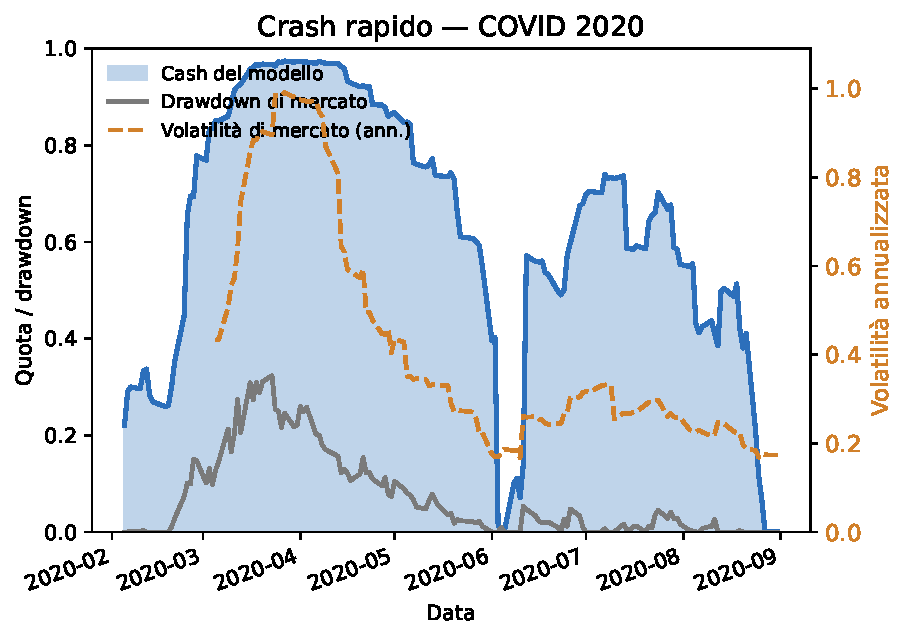
\includegraphics[width=\textwidth]{alloc_covid.pdf}
\caption{Crash rapido (COVID 2020)}
\label{fig:alloc-covid}
\end{subfigure}
\hfill
\begin{subfigure}{0.48\textwidth}\centering
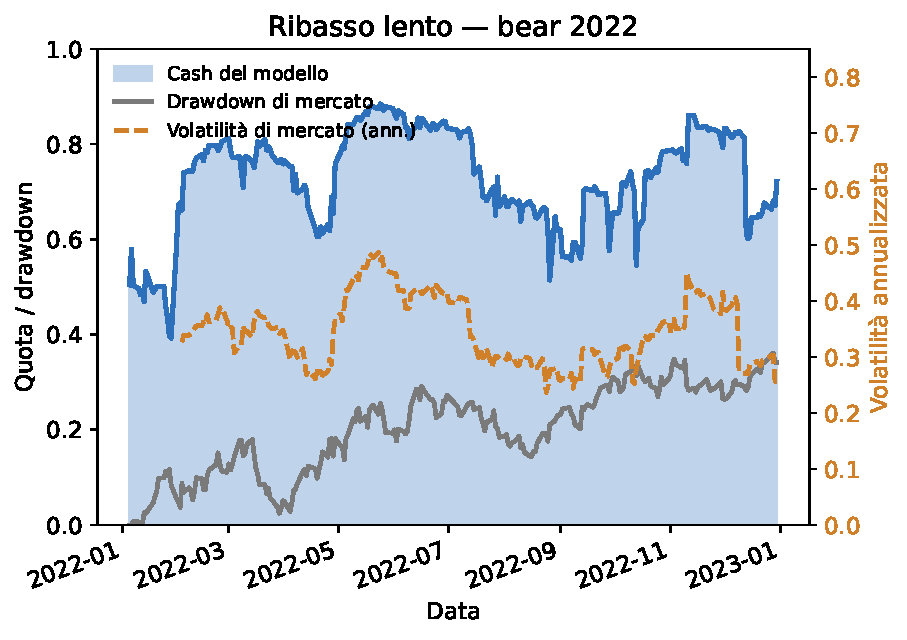
\includegraphics[width=\textwidth]{alloc_2022.pdf}
\caption{Ribasso lento (bear 2022)}
\label{fig:alloc-2022}
\end{subfigure}
\caption{Allocazione nel tempo: quota di liquidità del modello sovrapposta al drawdown/volatilità di mercato. Nel crash rapido (COVID) il cash sale in tempo; nel bear lento (2022) la volatilità resta bassa e la difesa arriva tardi.}
\label{fig:allocation-time}
\end{figure}


\subsection{Filo conduttore}
Ogni leva analizzata: $m_\theta$ calcolato, esponente stimato, regola in regime, non fornisce nulla che non si possa ottenere già scegliendo i parametri strutturali fissi ($\sigma_{\mathrm{target}}$ e esponente).
Il valore è completamente nella struttura, non nell'adattamento. 
La dipendenza dal regime è una caratteristica del mercato e non può essere utilizzata in tempo reale perché il regime è noto solo a posteriori. 
Il modello e la sua difesa si adattano a diversi universi, compresa la debolezza strutturale nei mercati lenti.





	\clearpage{\pagestyle{empty}\cleardoublepage}

    
	\chapter{Applicazione Mobile}
    \thispagestyle{chapterplain}
    \label{chap:applicazione}
	% !TEX root = main.tex
\section{Dettagli implementativi}
L'applicazione adotta un'architettura local-first cioè tutta l'elaborazione dei dati e le funzioni principali dell'app come il calcolo dei pesi e l'inferenza del modello avvengono sul dispositivo, l'unica interazione con la rete è il download periodico dei prezzi. I motivi dietro questa scelta sono:
\begin{itemize}
    \item \textbf{Privacy e autonomia}: i portafogli dell'utente, le allocazioni e i risultati non lasciano mai il dispositivo.
    \item \textbf{Funzionamento offline}: dopo la prima sincronizzazione l'app resta completamente utilizzabile anche senza connessione in quanto tutti i dati utili al suo funzionamento risiedono in un database locale.
    \item \textbf{Costo nullo di infrastruttura}: non essendoci un backend da mantenere, l'aggiornamento dei dati è delegato a un servizio di automazione gratuito, evitando qualsiasi hosting dedicato.

\end{itemize}
In sostanza c'è un separazione tra due sottosistemi: una pipeline di produzione del dato e un sottosistema di consumo e persistenza.
\subsubsection{Sorgente e struttura del dato}
\label{sec:sorgente e struttura del dato}
I dati di mercato sono ottenuti da Yahoo Finance tramite la libreria \lstinline{yfinance}. 
L'universo scaricato è l'intero indice S\&P500: l'elenco dei ticker è estratto a runtime dalla pagina di Wikipedia dell'indice, in modo da garantire l'aggiornamento automatico della composizione qualora dovesse cambiare nel tempo, nel caso in cui Wikipedia non dovesse essere raggiungibile viene usata una lista statica dei titoli nell'S\&P500.
Per ogni titolo viene acquisita una storia di tre anni di dati giornalieri, con la modalità \lstinline{auto_adjust = True} come per il modello. Le feature che vengono conservate sono le quattro feature di mercato utilizzate dal modello cioè high, low, close e VIX, l'open non viene memorizzata in quanto non viene utilizzata da alcun metodo. 
Il download avviene un ticker alla volta e non in blocco, in questo modo vengono prodotte serie a indice singolo più semplici e robuste da elaborare, e permette di isolare i fallimenti.
\subsubsection{Pipeline di aggiornamento automatico}
L'aggiornamento è affidato a un workflow di GitHub Actions, l'esecuzione avviene alle 22:00 UTC nei giorni feriali, ovvero dopo la chiusura del mercato statunitense. Il workflow:
\begin{enumerate}
    \item predispone un ambiente Python ed installa le dipendenze;
    \item esegue lo script di download, che produce il dataset;
    \item effettua il commit del dataset aggiornato nel repository.
\end{enumerate}
Il repository Git assume il ruolo di archivio versionato dei dati e punto di distribuzione verso i client.
Con tutti gli storici dei 503 titoli però esso raggiunge dimensioni di circa 33MB che è una dimensione molto grande per essere scaricata sui dispositivi mobili.
\subsection{Datasets}
\label{sec:datasets}
Il Dataset è in formato JSON, con due collezzioni principali: \lstinline{prices} e \lstinline{market}. 
Per questo motivo viene applicata una conversione gzip al momento della generazione del dataset: lo script genera accanto al JSON una versione compressa che pesa circa 5,4MB. 
La versione gzip è quella effettivamente usata, lato client la decompressione avviene attraverso la libreria \lstinline{fflate}, in javascript puro.

\subsubsection{Database locale}
\label{subsec:database locale}
Sul dispositivo i dati vengono racchiusi in un database SQLite, interrogato tramite l'ORM tipizzato Drizzle. 
Lo schema è minimale e normalizzato, ed è diviso nelle seguenti tabelle:
\begin{figure}[H]
  \centering
  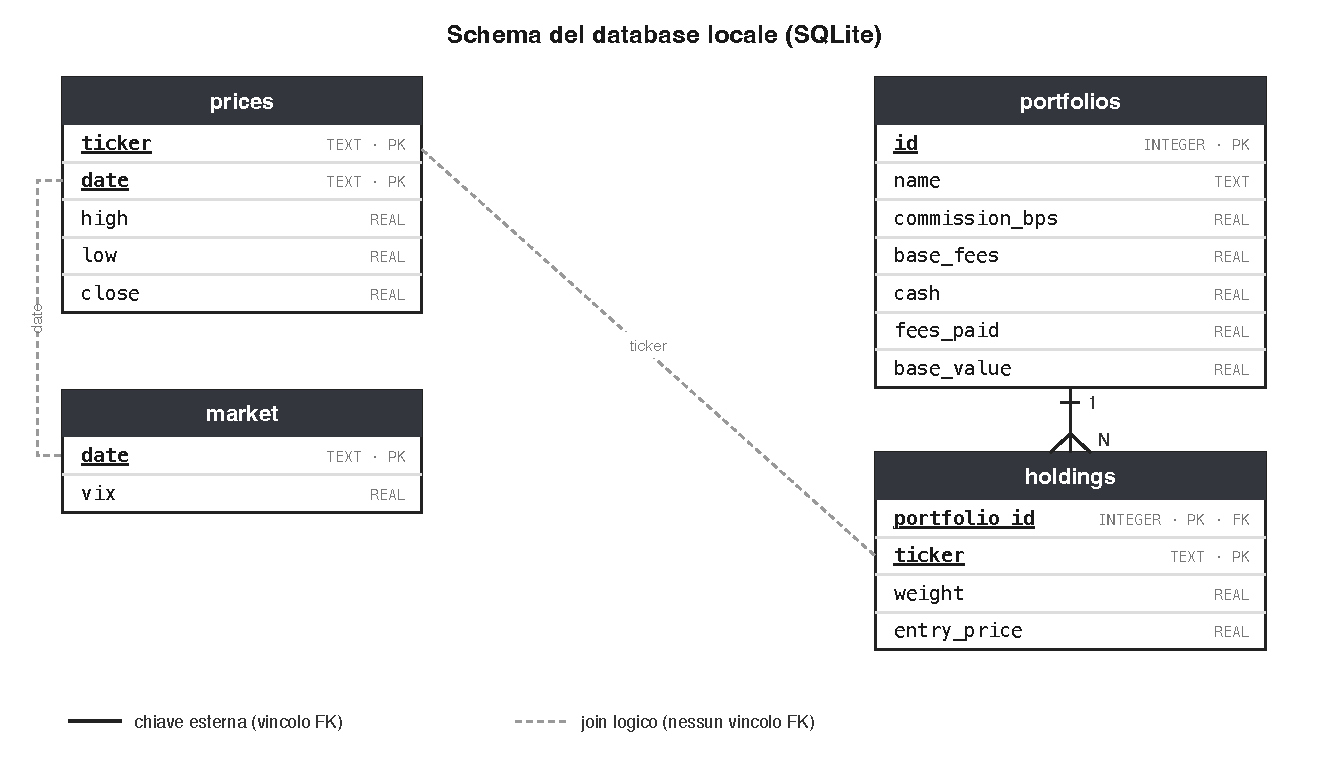
\includegraphics[width=0.95\textwidth]{er_diagram.pdf}
  Le chiavi primarie composte
  \texttt{(ticker,\,date)} e \texttt{(portfolio\_id,\,ticker)}
  impediscono che ci siano dati duplicati.
  L'unica relazione con vincolo di integrità
  referenziale è \texttt{holdings.portfolio\_id} $\rightarrow$
  \texttt{portfolios.id}.
  \label{fig:er-schema}
\end{figure}

SQLite su dispositivi mobili ha un limite di variabili che può gestire con un'unica query.
Per risolvere questo problema i dati vengono divisi in array da al massimo 500 elementi ciascuno.
I dati vengono quindi inseriti un blocco alla volta all'interno del database in modo da evitare errori.

L'evoluzione dello schema è gestita in maniera standard tramite migrazioni versionate, ovvero degli script sequenziali che modificano la struttura dei dati per adattarla ai requisiti del software.
Queste migrazioni vengono generate in fase di sviluppo e applicate automaticamente all'avvio, prima di ogni accesso ai dati. 
Un registro interno al database memorizza lo storico degli aggiornamenti assicurando che ogni migrazione venga applicata una sola volta.
In questo modo se il database è già allineato all'ultima versione l'aggiornamento si conclude senza eseguire nessuna istruzione.

\subsubsection{Sincronizzazione lato applicazione}

All'avvio, dopo le migrazioni, l'app esegue la procedura di sincronizzazione, che svolge tre operazioni fondamentali.
\begin{itemize}
  \item \textbf{Limitazione di frequenza}: una tabella di servizio conserva la data dell'ultima sincronizzazione e se coincide con quella odierna impedisce che vengano fatte altre sincronizzazioni.
  \item \textbf{Inserimento idempotente}: come descritto nella sezione precedente i dati vengono inseriti a blocchi.
  In caso di conflitto sulle chiavi primarie la riga esistente viene aggiornata con i valori
  piu' recenti. In questo modo si evitano duplicazioni di dati.
  \item \textbf{Finestra temporale mobile}: ad ogni sincronizzazione vengono scaricati gli ultimi tre anni di storico. 
  Si scaricano gli interi tre anni perché \lstinline{yfinance} con \lstinline{auto_adjust=True} aggiorna i prezzi compresi quelli passati ad ogni split e dividendo, quindi vanno sovrascritti.
  Per tenere lo spazio occupato costante vengono eliminati di volta in volta tutti i record corrispondenti a date precedenti alla prima data nel dataset scaricato.
\end{itemize}

\subsubsection{Inizializzazione e primo avvio}

L'applicazione include un seed iniziale di dati impacchettati nel bundle per garantire l'usabilità anche in assenza di rete alla prima apertura. 
Al primissimo avvio, se la tabella dei prezzi è vuota, il seed la popola. 
Successivamente la sincronizzazione allinea il contenuto alla versione più recente. 
Le tre fasi di sincronizzazione avvengono con frequenze diverse: le migrazioni sono verificate a ogni avvio ma applicate una sola volta, il seed viene eseguito solo a database vuoto, la sincronizzazione al più una volta al giorno.

\subsubsection{Limiti}
Si espongono in questa sezione limiti progettuali dell'app.
I dati vengono scaricati solo una volta al giorno e sono i prezzi a chiusura del mercato, non ci sono quindi dati in tempo reale.
L'API di \lstinline{yfinance} si appoggia a end-point non ufficiale di Yahho Finance, il servizio può cambiare senza preavviso e richiederebbe manutenzione dello script.
La distribuzione via repository nn è pensata come canale ad alto volume, funziona bene per essere usata da pochi utenti ma se diventano migliaia non reggerebbe la concorrenza.

\subsection{Esecuzione del modello on-device}
\label{subsec:inferenza-onnx}

Il modello discusso nella sezione~\ref{sec:modello} viene addestrato in Python ed esportato in formato ONNX (Open Neural Network Exchange).
ONNX è uno standard e serve a disaccoppiare il framework di addestramento dal motore di esecuzione.
In questo modo è possibile far girare il modello in un ambiente React Native direttamente sul dispositivo.

L'inferenza quindi avviene in locale utilizzando la libreria \lstinline{onnxruntime-react-native} che esegue il modello sulla CPU del dispositivo.
Non è previsto alcun server di inferenza: i dati dell'utente non lasciano mai il dispositivo e l'intera app funziona anche offline.


Il file ONNX del modello è incluso come asset nel bundle dell'applicazione.
All'avvio viene creata una sola sessione di inferenza che viene conservata in un singleton di modulo e riutilizzata per tutte le previsioni successive. 
Il costo di caricamento del modello si paga quindi una volta sola, in background, senza bloccare l'interfaccia. 
Un meccanismo di guardia impedisce inizializzazioni concorrenti.

Ogni previsione segue tre passi:
\begin{enumerate}
  \item si costruiscono i tre tensori di input:\lstinline{features}, \lstinline{prev_weights} e \lstinline{risk_state}, in formato \lstinline{float32};
  \item si esegue la sessione con \lstinline{session.run(feeds)};
  \item si legge il tensore di output \lstinline{portfolio_weights}, i pesi del
  portafoglio che sommano a $1$.
\end{enumerate}

Questa procedura è usata in due funzionalità diverse.
Viene usata per l'allocazione in tempo reale quando l'utente applica il metodo al suo portafoglio facendo partire una previsione usando i dati più recenti.
E viene usata anche per il backtest in cui il modello viene interrogato ad ogni ribilanciamento.



     \chapter{Formule}
    \thispagestyle{chapterplain}
	\label{chap:Formule}
	% !TEX root = main.tex
\section{Strategie}
\label{set:strategie}

   \subsection{Inverse Volatility}
\label{sec:inverse_volatility}

L'idea fondamentale di questa strategia consiste nell'assegnare il capitale in modo \textbf{inversamente proporzionale} alla volatilità di ciascun asset, penalizzando i titoli più nervosi e premiando quelli più stabili.

Il calcolo dell'allocazione si articola in tre passaggi principali:
\begin{enumerate}
    \item \textbf{Misura del rischio}: Per ogni asset $i$, si calcola la volatilità storica $\sigma_i$ applicando la deviazione standard campionaria sui rendimenti.
    \item \textbf{Inversione}: Si calcola il reciproco della volatilità $\frac{1}{\sigma_i}$. Se un titolo presenta un'elevata volatilità, il suo inverso risulterà contenuto; viceversa, per un titolo stabile il reciproco assume un valore più elevato.
    \item \textbf{Normalizzazione}: Si divide l'inverso della volatilità del singolo asset per la somma degli inversi di tutti gli asset del portafoglio, garantendo che la somma dei pesi $w_i$ sia pari a $1$ ($100\%$ del capitale allocato).
\end{enumerate}

La formula matematica per il calcolo del peso $w_i$ dell'asset $i$-esimo è definita come:

\begin{equation}
    w_i = \frac{\frac{1}{\sigma_i}}{\sum_{j=1}^{N} \frac{1}{\sigma_j}}
\end{equation}

dove:
\begin{itemize}
    \item $w_i$ è il peso percentuale assegnato all'asset $i$-esimo nel portafoglio;
    \item $\sigma_i$ è la deviazione standard campionaria dei rendimenti dell'asset $i$;
    \item $N$ è il numero totale di asset presenti nel portafoglio;
    \item $\sum_{j=1}^{N} \frac{1}{\sigma_j}$ rappresenta la somma degli inversi delle volatilità di tutti gli asset (fattore di normalizzazione).
\end{itemize}

Nel codice TypeScript riportato, vengono inseriti dei controlli difensivi: se la deviazione standard di un asset è pari a zero ($\sigma_i = 0$), il suo valore reciproco viene impostato a $0$ per evitare la divisione per zero. Allo stesso modo, se la somma totale degli inversi risulta nulla, la funzione restituisce un vettore di pesi azzerati.

\begin{lstlisting}[language=TypeScript, caption={Implementazione dell'algoritmo Inverse Volatility.}, label={lst:inverse_volatility}]
export function inverseVolatility(returnsByAsset: number[][]): number[] {
  // 1. Calcolo del reciproco della volatilita per ogni asset
  const inv = returnsByAsset.map((r) => {
    const s = sampleStd(r);
    return s === 0 ? 0 : 1 / s; // Guard divisione per zero
  });

  // 2. Somma totale dei reciproci
  const tot = inv.reduce((a, b) => a + b, 0);
  if (tot === 0) return inv.map(() => 0);

  // 3. Normalizzazione a somma 1 (100% del capitale)
  return inv.map((x) => x / tot);
}
\end{lstlisting}

    \subsection{Kelly Criterion}
\label{sec:kelly_criterion}

Il criterio di Kelly calcola l'esposizione ottimale di capitale per massimizzare il tasso di crescita logaritmico del portafoglio nel tempo. La formula classica in forma matriciale è definita come:

\begin{equation}
    \mathbf{f}^* = \mathbf{\Sigma}^{-1} \boldsymbol{\mu}
\end{equation}

\begin{itemize}
    \item $\mathbf{f}^*$ è il vettore dei pesi ideali delle posizioni;
    \item $\mathbf{\Sigma}^{-1}$ è l'inversa della matrice di covarianza dei rendimenti;
    \item $\boldsymbol{\mu}$ è il vettore dei rendimenti attesi (\textit{expected returns}).
\end{itemize}

A questa formulazione teorica vengono applicate quattro modifiche pratiche. La formula pura, infatti, risulta estremamente sensibile agli errori di stima degli input (\textit{garbage in, garbage out}) e tende a generare una leva finanziaria eccessivamente aggressiva ed instabile.

Le quattro modifiche apportate sono le seguenti:

\begin{enumerate}
    \item \textbf{Regolarizzazione della Matrice (\textit{Covariance Shrinkage})}: Se due o più titoli presentano un comportamento fortemente correlato o se il numero di campioni storici è ridotto, la matrice di covarianza diventa singolare (o quasi singolare). L'inversione di una tale matrice in JavaScript comporta gravi errori di precisione numerica o il blocco dell'applicazione. Per garantire la stabilità computazionale, viene applicata una regolarizzazione sui parametri fuori dalla diagonale principale:
    \begin{equation}
        \mathbf{\Sigma}_{\text{shrunk}}(i, j) = 
        \begin{cases} 
            \mathbf{\Sigma}(i, j) & \text{se } i = j \quad \text{(diagonale principale: varianze inalterate)} \\ 
            (1 - \delta) \cdot \mathbf{\Sigma}(i, j) & \text{se } i \neq j \quad \text{(fuori diagonale: covarianze ridotte del } 15\% \text{)}
        \end{cases}
    \end{equation}
    In questo modo, i titoli appaiono leggermente meno correlati tra loro, garantendo un'inversione matriciale numericamente stabile.

    \item \textbf{Scalamento Half-Kelly}: Dopo aver calcolato il vettore $\mathbf{f}^*$, si applica uno scalamento dimezzandone i valori:
    \begin{equation}
        \mathbf{f}_{\text{half}} = \frac{1}{2} \mathbf{f}^*
    \end{equation}
    Lo scopo è mitigare i \textit{drawdown} estremi causati da una leva eccessiva. Dimezzare le posizioni riduce la varianza complessiva del portafoglio del $75\%$, sacrificando solo una quota minima del tasso di crescita teorico.

    \item \textbf{Vincolo Long-Only}: La formula originale restituisce sia valori positivi che negativi (dove un valore positivo come $+0.4$ indica l'acquisto del titolo col $40\%$ del capitale, mentre un valore negativo come $-0.25$ suggerisce la vendita allo scoperto per il $25\%$). Poiché lo \textit{short selling} richiede garanzie sui margini e autorizzazioni complesse, si è scelto di eliminare le posizioni corte applicando una funzione di taglio:
    \begin{equation}
        f_i^{\text{long}} = \max\left(0, f_{\text{half}, i}\right)
    \end{equation}

    \item \textbf{Cap della Leva Massima (\textit{Leverage Ceiling})}: Il criterio di Kelly tende ad adottare una strategia di leva molto aggressiva. Si è stabilito quindi un limite massimo alla leva finanziaria $L_{\max} = 2$. Se l'esposizione lorda complessiva $L = \sum f_i^{\text{long}}$ supera tale soglia, i pesi vengono riallocati proporzionalmente:
    \begin{equation}
        \mathbf{f}_{\text{finale}} = 
        \begin{cases} 
            \mathbf{f}^{\text{long}} & \text{se } L \le L_{\max} \\ 
            \mathbf{f}^{\text{long}} \cdot \frac{L_{\max}}{L} & \text{se } L > L_{\max} 
        \end{cases}
    \end{equation}
\end{enumerate}

Nel Listing viene riportata l'implementazione in TypeScript della funzione descritta.

\begin{lstlisting}[language=TypeScript, caption={Implementazione dell'algoritmo di Kelly Multi-Asset.}, label={lst:kelly_criterion}]
export function kelly(
  mu: number[],
  cov: number[][],
  opts: { shrink?: number; halfKelly?: boolean; maxLeverage?: number } = {},
): number[] {
  const { shrink = 0.15, halfKelly = true, maxLeverage = 2 } = opts;

  // 1. Regolarizzazione della matrice (Shrinkage)
  const shrunk = cov.map((row, i) =>
    row.map((v, j) => (i === j ? v : (1 - shrink) * v)),
  );
  const covInv = invertMatrix(shrunk);

  // 2. Calcolo f* = Sigma^-1 * mu
  let f = matVec(covInv, mu); 

  // 3. Vincolo Long-Only
  f = f.map((x) => Math.max(0, x)); 

  // 4. Cap della Leva Massima
  const gross = f.reduce((a, b) => a + b, 0);
  if (gross > maxLeverage) f = f.map((x) => (x * maxLeverage) / gross); 

  // 5. Half-Kelly
  if (halfKelly) f = f.map((x) => x / 2); 

  return f; // Esposizioni (il capitale non allocato rimane in Cash)
}
\end{lstlisting}

\subsection{Target Volatility}
\label{sec:target_volatility}

L'obiettivo della strategia di \textit{Target Volatility} (o \textit{Volatility Targeting}) è controllare il rischio complessivo del portafoglio, mantenendo la sua volatilità stimata entro una soglia predefinita ($\sigma_{\text{target}}$). Se la volatilità del portafoglio di partenza supera tale limite, l'algoritmo riduce proporzionalmente l'esposizione su tutti i titoli, allocando la quota rimanente di capitale in liquidità (\textit{Cash}).

L'implementazione segue tre passaggi principali:

\begin{enumerate}
    \item \textbf{Volatilità del portafoglio (giornaliera e annualizzata)}: Si calcola prima la deviazione standard giornaliera mediante la forma quadratica della matrice di covarianza $\mathbf{\Sigma}$ e del vettore dei pesi base $\mathbf{w}_{\text{base}}$, per poi annualizzarla moltiplicando per la radice dei giorni lavorativi ($\sqrt{252}$):
    \begin{equation}
        \sigma_{\text{port, giornaliera}} = \sqrt{\mathbf{w}_{\text{base}}^T \mathbf{\Sigma} \mathbf{w}_{\text{base}}}
    \end{equation}
    \begin{equation}
        \sigma_{\text{port, annua}} = \sigma_{\text{port, giornaliera}} \times \sqrt{252}
    \end{equation}

    \item \textbf{Fattore di scalamento}: Viene calcolato il coefficiente di riduzione $\text{scale}$:
    \begin{equation}
        \text{scale} = \min\left(1, \; \frac{\sigma_{\text{target}}}{\sigma_{\text{port, annua}}}\right)
    \end{equation}
    L'utilizzo dell'operatore $\min(1, \dots)$ impedisce l'impiego della leva finanziaria, evitando che l'algoritmo aumenti l'esposizione complessiva oltre il $100\%$ del capitale nei periodi di bassa volatilità. Inoltre, il rapporto $\frac{\sigma_{\text{target}}}{\sigma_{\text{port, annua}}}$ esegue un de-risking automatico nelle fasi di elevata turbolenza di mercato: quando la volatilità annua registra picchi improvvisi, il fattore $\text{scale}$ si riduce automaticamente, vendendo quote dei titoli per rifugiarsi nella liquidità e proteggere il portafoglio da ampi \textit{drawdown}.

    \item \textbf{Pesi scalati}: Ogni peso dell'allocazione base viene ridimensionato applicando il fattore di scalamento:
    \begin{equation}
        \mathbf{w}_{\text{finale}} = \mathbf{w}_{\text{base}} \times \text{scale}
    \end{equation}
\end{enumerate}

La funzione gestisce anche il caso limite in cui la volatilità annualizzata sia nulla ($\sigma_{\text{port, annua}} = 0$), impostando il fattore di scala a $1$ per evitare divisioni per zero.

\begin{lstlisting}[language=TypeScript, caption={Implementazione dell'algoritmo Target Volatility.}, label={lst:target_volatility}]
export function targetVolatility(
  wBase: number[],
  cov: number[][],
  sigmaTargetAnnual = 0.097, // 2.8% mensile ~ 9.7% annuo
): number[] {
  // 1. Calcolo della volatilita giornaliera ed annualizzata del portafoglio
  const sigmaDaily = Math.sqrt(quadForm(wBase, cov));
  const sigmaAnnual = sigmaDaily * Math.sqrt(252);

  // 2. Calcolo del fattore di scalamento (cap a 1, no leva)
  const scale =
    sigmaAnnual === 0 ? 1 : Math.min(1, sigmaTargetAnnual / sigmaAnnual);

  // 3. Applicazione del fattore ai pesi (il capitale rimanente va in Cash)
  return wBase.map((w) => w * scale);
}
\end{lstlisting}
	\clearpage{\pagestyle{empty}\cleardoublepage}

	\chapter{Conclusioni}
    \thispagestyle{chapterplain}
    \label{chap:conclusioni}
	% !TEX root = main.tex
\section{Discussione: un risultato atteso nella letteratura}


I risultati ottenuti da questi esperimenti non sono esiti isolati. 
Il modello non riesce ad ottenere dalle feature segnali abbastanza forti da riuscire 
a sbloccare una sorta di previsione o intelligenza che gli permetta di battere 
la formula su cui si basa.
Questo accade perché l'unico segnale che il modello riesce a sfruttare è quello della volatilità,
ed proprio il dato principale su cui si basa la formula statica di partenza.
La volatilità infatti può essere predetta: essa infatti tende ad addensarsi e susseguirsi, fasi ad altà volatilità sono seguite da altre fasi simili
e ugualmente succede per le fasi di bassa volatilità. Questa proprietà è ben documentata e rende la volatilità un segnale stimabile
in anticipo.
E proprio questa caratteristica che ha portato al basare il modello sul volatility timing utilizzando la formula del volatility targeting di Moreira Muir.
Il segnale mancante che la formula non ha e che permetterebbe al modello di battere la formula di partenza
è la predizione della direzione del mercato. 
Questo segnale però è già stato dimostrato non essere ottenibile, la prevedibilità dei rendimenti azionari è notoriamente debole e instabile.
Nel paper \citet{goyal2024comprehensive} infatti si dimostra che fuori-campione la quasi totalità
delle strategie e delle variabili proposte dalla letteratura accademica fallisce nel battere 
una previsione banale basata sulla semplice media storica. In sostanza non ci sono ancora
modi per riuscire a prevedere la direzione futura del mercato. 
L'impossibilità di prevedere la direzione del mercato specialmente nel DRL è data dal fatto che la maggior parte 
delle informazioni che si possono ottenere dagli scambi giornalieri è quasi interamente rumore. Quando i modelli cercano di estrarre delle 
informazioni rilevanti da questi dati finiscono solo per fare over-fitting sul backtest in cui è stato addestrato.
Questo spiega anche perché le prove fuori campione di modelli che sono stati presentati come funzionali in campione si dimostrano 
per la maggior parte un buco nell'acqua \citet{bailey2014pseudo}.

Tirando le conclusioni il fatto che il modello converga sulla formula di partenza non è del tutto un fallimento.
Può essere visto come un esito informativo, esso sebbene confermi che il valore della strategia risieda nella sua struttura 
anziché nella parte appresa, dimostra che l'agente in assenza di segnale sfruttabile ha imparato la scelta corretta, ovvero riprodurre la regola ottimale 
evitando di inseguire pattern inconcludenti e degenrare.



Infine va riconosciuto il confine di questa conclusione. \citet{gu2020empirical}
documentano che il machine learning \emph{aggiunge} valore nell'asset pricing
empirico, ma nella dimensione \emph{cross-sectional} --- la selezione tra molti
titoli --- e attraverso segnali come momentum, liquidita' e volatilita'. E'
esattamente la leva che qui e' stata congelata: il valore dell'apprendimento, se
esiste in questo dominio, va cercato nella selezione cross-asset e in universi
meno efficienti, non in un overlay piu' sofisticato sulla sola esposizione. Il
contributo di questo lavoro non e' dunque dimostrare che l'apprendimento batte una
regola, ma quantificare con rigore, tramite ablation e controlli, il limite
dell'adattivita' appresa in un regime a basso rapporto segnale/rumore.

\paragraph{Limiti.} Le conclusioni valgono per l'universo (large-cap S\&P~500,
selezione congelata), i periodi e gli obiettivi considerati. Su mercati
strutturalmente meno efficienti, o in problemi dove la selezione cross-asset e'
determinante, il margine per l'apprendimento potrebbe riaprirsi.

\paragraph{Contributo di questo lavoro.}
La maggior parte dei lavori che aplicano il reinforcement learning alla gestione del portafoglio presentano un solo backtest
Il problema è che facendo molti backtest con varie combinazioni è facile trovarne una che nel suo campione si dimostra vincente
per puro caso. Tuttavia questo risultato vincente nel backtest in campione non si traduce ugualmente fuori campione come dimostrato da \citet{bailey2014pseudo}.
In questo lavoro sono state testate diverse configurazioni su vari panieri e periodi temporali, testando il modello e isolando le sue parti aprendibili per capirne i valori e i problemi di ognuna.
Le accortezze che sono state fatte sono:
\begin{itemize}
    \item L'apprendimento non sostituisce la strategia del volatility targeting e questo permette un confronto pulito tra ciò che la rete impara e quello che la formula fornisce.
    \item Si è scelto di valutare ogni componente apprendibile isolandolo e confrontandolo con la sua controparte strutturale.
    \item Le metriche sono riportate come mediana multi-seed, non si è selezionato l'esito più favorevole.
    \item Verifica di generalità in cui il modello è stato testato su panieri mai visti in addestramento.
\end{itemize}

Infine tutti quelle che sembravano azioni vantaggiose del modello sono state analizzate per capirne le cause, e se fossero o meno date da un effetiva intelligenza del modello o semplicemente dalla sua maggiore conservatività.


Il contributo, in sintesi, non è dimostrare che l'apprendimento batte una regola, ma \textbf{quantificare con rigore, tramite ablation e controlli, il limite dell'adattività appresa} in un dominio a basso rapporto segnale/rumore e spiegarne la ragione economica.

1 Stato dell'arte con parte finale dedicata alle motivazioni
2 Progettazione dataset e metodi
3 Implementazione
4 risultati
5 Applicazione mobile comprensiva di workflow della UI e lati salienti dell'Implementazione
6 Conclusioni


    
    \pagestyle{plain}
    \cleardoublepage
    \setcounter{page}{1}
    \renewcommand{\thepage}{B\arabic{page}}
    \bibliographystyle{plainnat}
    \addcontentsline{toc}{chapter}{Bibliography}
    \bibliography{references}

\end{document}

